% Presets
\setbeamertemplate{itemize/enumerate body begin}{\footnotesize}
\setbeamertemplate{itemize/enumerate subbody begin}{\footnotesize}




%%%%%%%%%%%%%%%%%%%%%%%%%%%%%%%%%%%%%%%%%%%%%%%%%%%%%%%%%%%%%%%%%%%%%%%%%%%%%%%%%%%%%%%%%%%%%%%%%%%%%%%%%%%%%%%%%%%%%%%%%%%%
% Title page
%%%%%%%%%%%%%%%%%%%%%%%%%%%%%%%%%%%%%%%%%%%%%%%%%%%%%%%%%%%%%%%%%%%%%%%%%%%%%%%%%%%%%%%%%%%%%%%%%%%%%%%%%%%%%%%%%%%%%%%%%%%%


% Create background image
{\setbeamertemplate{sidebar right}{\llap{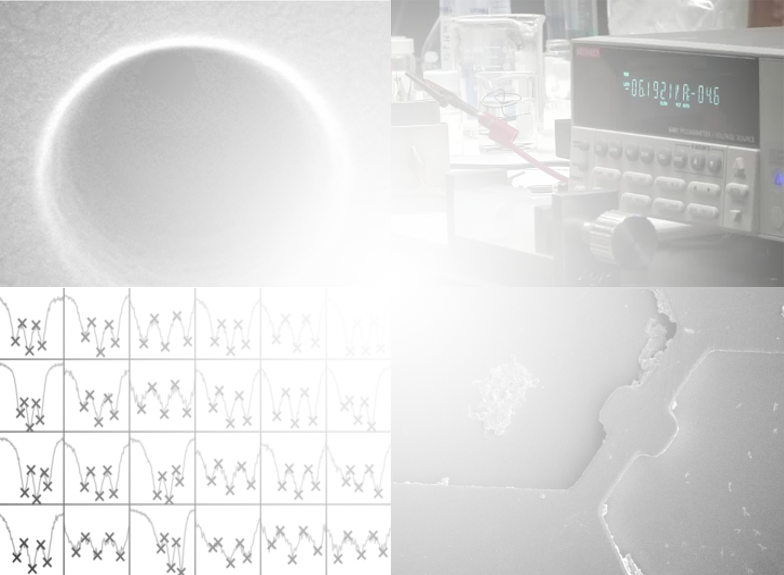
\includegraphics[width=\paperwidth,height=\paperheight]{title_image.png}}}
\begin{frame}[c]
 \begin{center}
  

  
  % Title
  \Huge{
	\textcolor{gray0}{Resistive-pulse sensing at the micro- and nanoscale}
  }
  
  
  % Name --- Institution
  \vspace{.25in}
  {\Large 
	\textcolor{gray1}{Preston Hinkle} \hspace{.5in} 
\includegraphics[height=1em]{uci_wordmark.png}
  }
  
  
  % Talk location
  \vspace{.5in}
  {\small
	\textit{\today}
  }
  
  
  
 \end{center}

\end{frame}
}



%%%%%%%%%%%%%%%%%%%%%%%%%%%%%%%%%%%%%%%%%%%%%%%%%%%%%%%%%%%%%%%%%%%%%%%%%%%%%%%%%%%%%%%%%%%%%%%%%%%%%%%%%%%%%%%%%%%%%%%%%%%%
% Outline
%%%%%%%%%%%%%%%%%%%%%%%%%%%%%%%%%%%%%%%%%%%%%%%%%%%%%%%%%%%%%%%%%%%%%%%%%%%%%%%%%%%%%%%%%%%%%%%%%%%%%%%%%%%%%%%%%%%%%%%%%%%%


\begin{frame}[c]{Outline}
 
	\begin{columns}[t]
		\begin{column}[T]{2.25in}
		
			\setbeamercovered{transparent}
			\begin{itemize}
				\item\only<1>{\textcolor{porestatsblack}{Resistive pulse sensing background}}\only<2,3,4>{\textcolor{ucigray0}{Resistive pulse sensing background}}
				\item\only<2>{\textcolor{porestatsblack}{Resistive pulse sensing of high-aspect ratio particles}}\only<1,3,4>{\textcolor{ucigray0}{Resistive pulse sensing of high-aspect ratio particles}}	
				\item\only<3,4>{\textcolor{porestatsblack}{Microscale resistive pulse sensing}}\only<1,2>{\textcolor{ucigray0}{Microscale resistive pulse sensing}}
				
					\begin{itemize}
						\item\only<3>{\textcolor{porestatsblack}{Simultaneous imaging and resistive pulse studies}}\only<1,2,4>{\textcolor{ucigray0}{Simultaneous imaging and resistive pulse studies}}
						\item\only<4>{\textcolor{porestatsblack}{Cancer cell deformability cytometry}}\only<1,2,3>{\textcolor{ucigray0}{Cancer cell deformability cytometry}}
					\end{itemize}
					
					
				
			\end{itemize}
			\setbeamercovered{invisible}
			
		\end{column}
		
		
		\begin{column}[T]{2.25in}
	
		
			% RP Background 1
			\onslide<1>{
				\begin{picture}(0,0)(0,0)
					\put(0,-180)
					{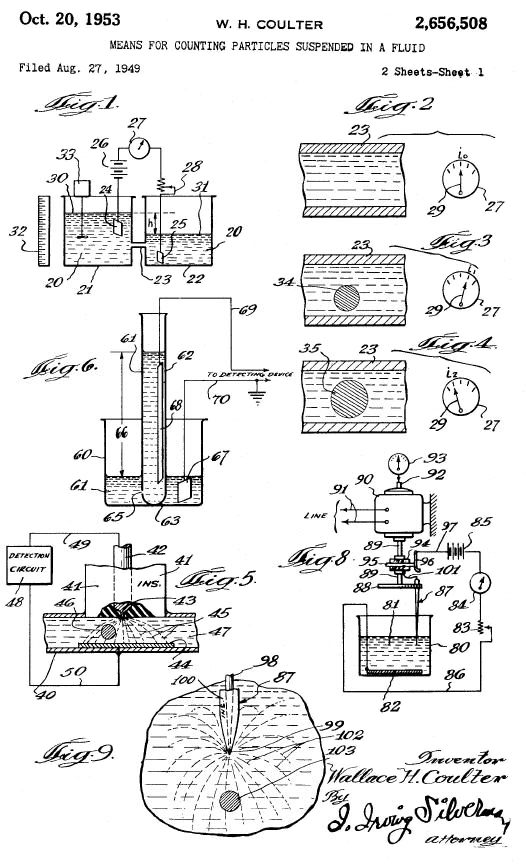
\includegraphics[width=2in]{coulter_patent_drawing}}
				\end{picture}
			}

		
			% Rods 1
			\onslide<2>{
				\begin{picture}(0,0)(0,0)
					\put(10,-30)
					{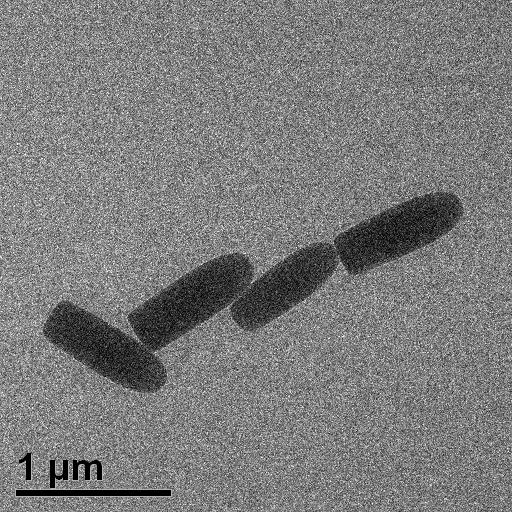
\includegraphics[width=1.25in]{shortrods}}
				\end{picture}
			}
			
			% Rods 2
			\onslide<2>{
				\begin{picture}(0,0)(0,0)
					\put(50,-125)
					{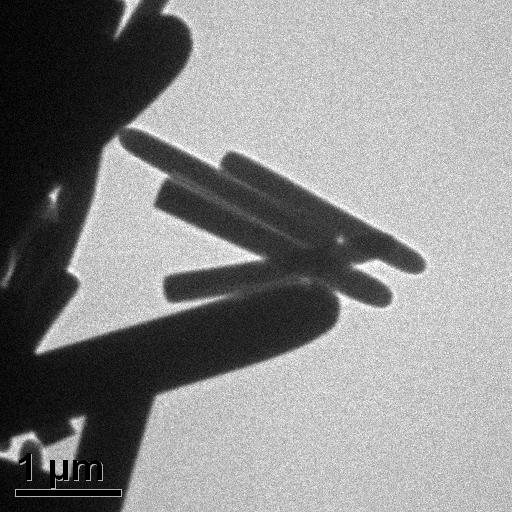
\includegraphics[width=1.25in]{longrods}}
				\end{picture}
			}
			
			
			% RPIM 1
			\onslide<3>{
				\begin{picture}(0,0)(0,0)
					\put(0, -65)
					{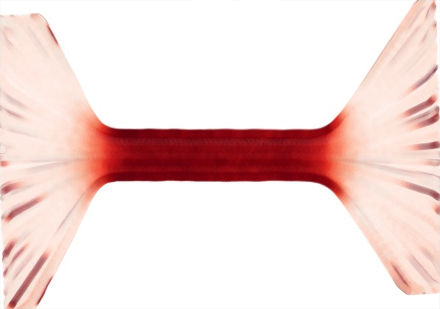
\includegraphics[width=2.25in]{resistancemap}}
				\end{picture}
			}
			
			% Cells
			\onslide<4>{
				\begin{picture}(0,0)(0,0)
					\put(0, -75)
					{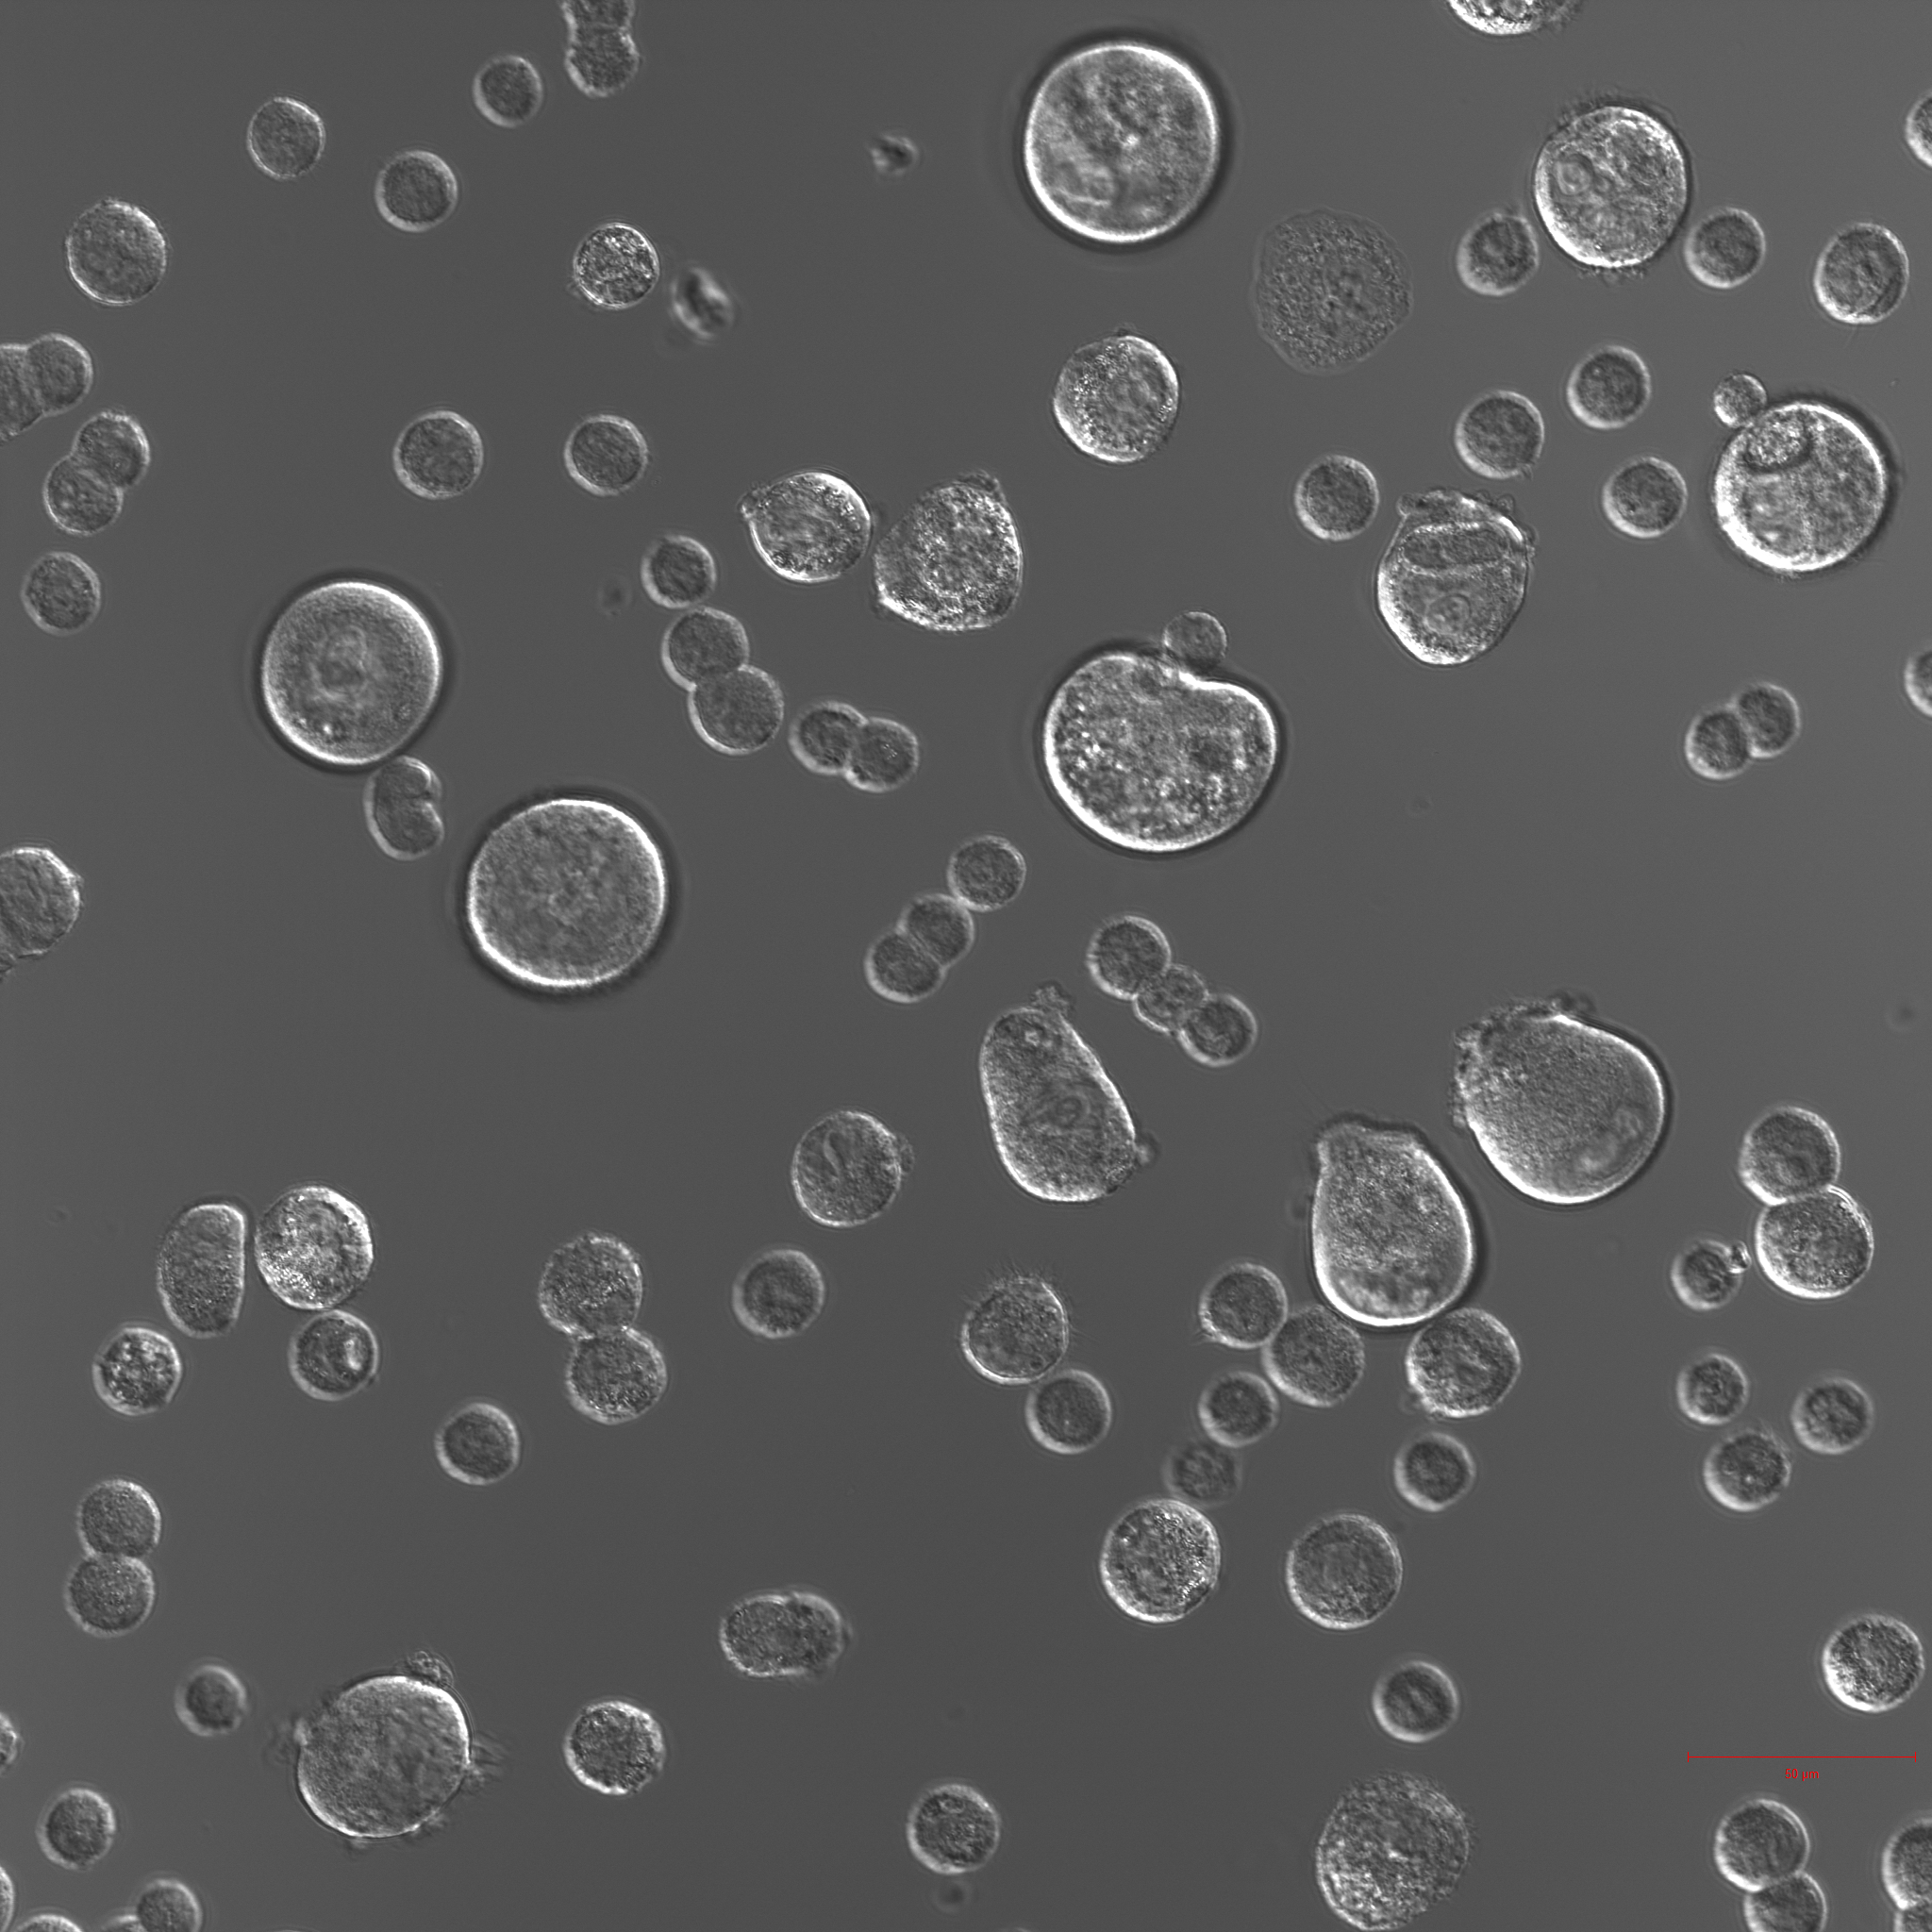
\includegraphics[width=2.25in]{cells}}
				\end{picture}
			}


			
			
		\end{column}
		
	\end{columns}

	
	
	
	
	
\end{frame}


%%%%%%%%%%%%%%%%%%%%%%%%%%%%%%%%%%%%%%%%%%%%%%%%%%%%%%%%%%%%%%%%%%%%%%%%%%%%%%%%%%%%%%%%%%%%%%%%%%%%%%%%%%%%%%%%%%%%%%%%%%%%
% Resistive pulse background title slide
%%%%%%%%%%%%%%%%%%%%%%%%%%%%%%%%%%%%%%%%%%%%%%%%%%%%%%%%%%%%%%%%%%%%%%%%%%%%%%%%%%%%%%%%%%%%%%%%%%%%%%%%%%%%%%%%%%%%%%%%%%%%


\begin{frame}[c]{}
	\begin{center}
		\textbf{Resistive pulse sensing background}
	\end{center}
\end{frame}



%%%%%%%%%%%%%%%%%%%%%%%%%%%%%%%%%%%%%%%%%%%%%%%%%%%%%%%%%%%%%%%%%%%%%%%%%%%%%%%%%%%%%%%%%%%%%%%%%%%%%%%%%%%%%%%%%%%%%%%%%%%%
% Resistive pulse background---description
%%%%%%%%%%%%%%%%%%%%%%%%%%%%%%%%%%%%%%%%%%%%%%%%%%%%%%%%%%%%%%%%%%%%%%%%%%%%%%%%%%%%%%%%%%%%%%%%%%%%%%%%%%%%%%%%%%%%%%%%%%%%


\begin{frame}[c]{Resistive pulse sensing---description}
	
	\begin{columns}[t]
		\begin{column}[T]{2.75in}
	
			\begin{itemize}
				\item Resistive pulse sensing (RP) is a method for single particle detection and characterization
				\item Works at any scale (nano, micro, milli, etc.)
				\item A diverse range of applications: red blood cell counting (several $\SI{}{\mu m}$, virus detection ($10-\SI{100}{\mu m}$, and DNA sequencing ($\sim\SI{1}{nm}$), among others
			\end{itemize}
	
		\end{column}
		
		\begin{column}[T]{1.75in}
			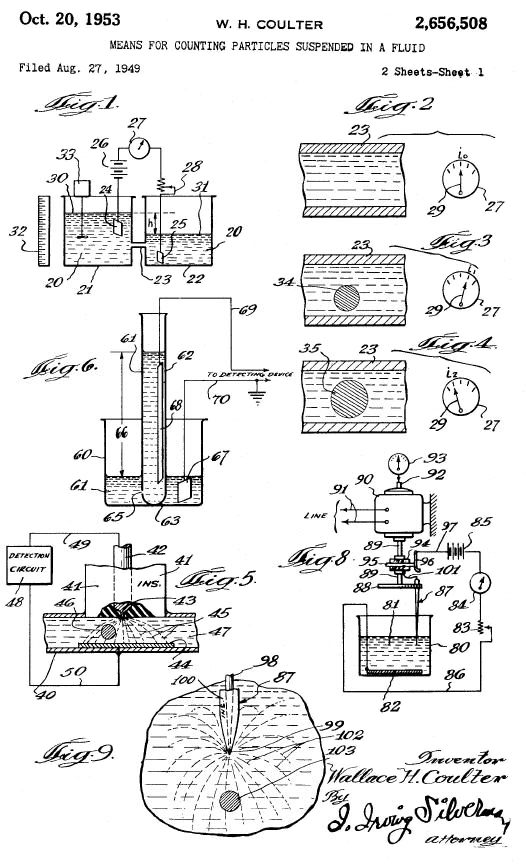
\includegraphics[width=1.75in]{coulter_patent_drawing.png}
		\end{column}
		
	\end{columns}

	
\end{frame}



%%%%%%%%%%%%%%%%%%%%%%%%%%%%%%%%%%%%%%%%%%%%%%%%%%%%%%%%%%%%%%%%%%%%%%%%%%%%%%%%%%%%%%%%%%%%%%%%%%%%%%%%%%%%%%%%%%%%%%%%%%%%
% Resistive pulse background---how does it work?
%%%%%%%%%%%%%%%%%%%%%%%%%%%%%%%%%%%%%%%%%%%%%%%%%%%%%%%%%%%%%%%%%%%%%%%%%%%%%%%%%%%%%%%%%%%%%%%%%%%%%%%%%%%%%%%%%%%%%%%%%%%%


\begin{frame}[c]{Resistive pulse sensing---how does it work?}

	\begin{columns}[t]
		\begin{column}[T]{2.75in}
	      
	

			\begin{tiny}
				\begin{itemize}
				
					\item A nanopore immersed in electrolyte solution acts as an ionic resistor
					\item Current-Voltage relationship follows Ohm's law $V=IR$
					\item When a particle enters the channel its resistance changes, yielding a pulse in the measured ionic current
					\item Pulse properties yield information on size, shape, charge, and concentration of particle
				\end{itemize}
			\end{tiny}
			
		\end{column}
		
		\begin{column}[T]{1.75in}
			{\centering
				\vspace{.5cm}
				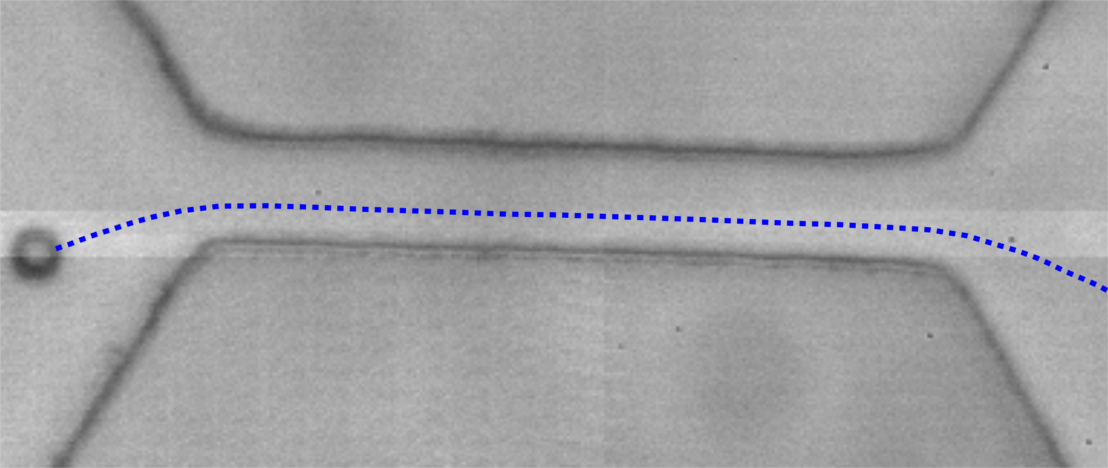
\includegraphics[width=1.5in]{singletrajectory} \\
				\vspace{.75cm}
				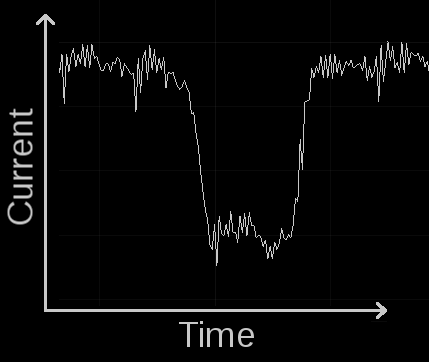
\includegraphics[width=1.5in]{singlerp} \\
				\par
			}
			
		\end{column}

	
	
	\end{columns}
	
\end{frame}




%%%%%%%%%%%%%%%%%%%%%%%%%%%%%%%%%%%%%%%%%%%%%%%%%%%%%%%%%%%%%%%%%%%%%%%%%%%%%%%%%%%%%%%%%%%%%%%%%%%%%%%%%%%%%%%%%%%%%%%%%%%%
% Resistive pulse background---system components
%%%%%%%%%%%%%%%%%%%%%%%%%%%%%%%%%%%%%%%%%%%%%%%%%%%%%%%%%%%%%%%%%%%%%%%%%%%%%%%%%%%%%%%%%%%%%%%%%%%%%%%%%%%%%%%%%%%%%%%%%%%%


\begin{frame}[c]{Resistive pulse sensing---system components}
	%\begin{picture}(0,0)(0,0)
		%\put(90,-125){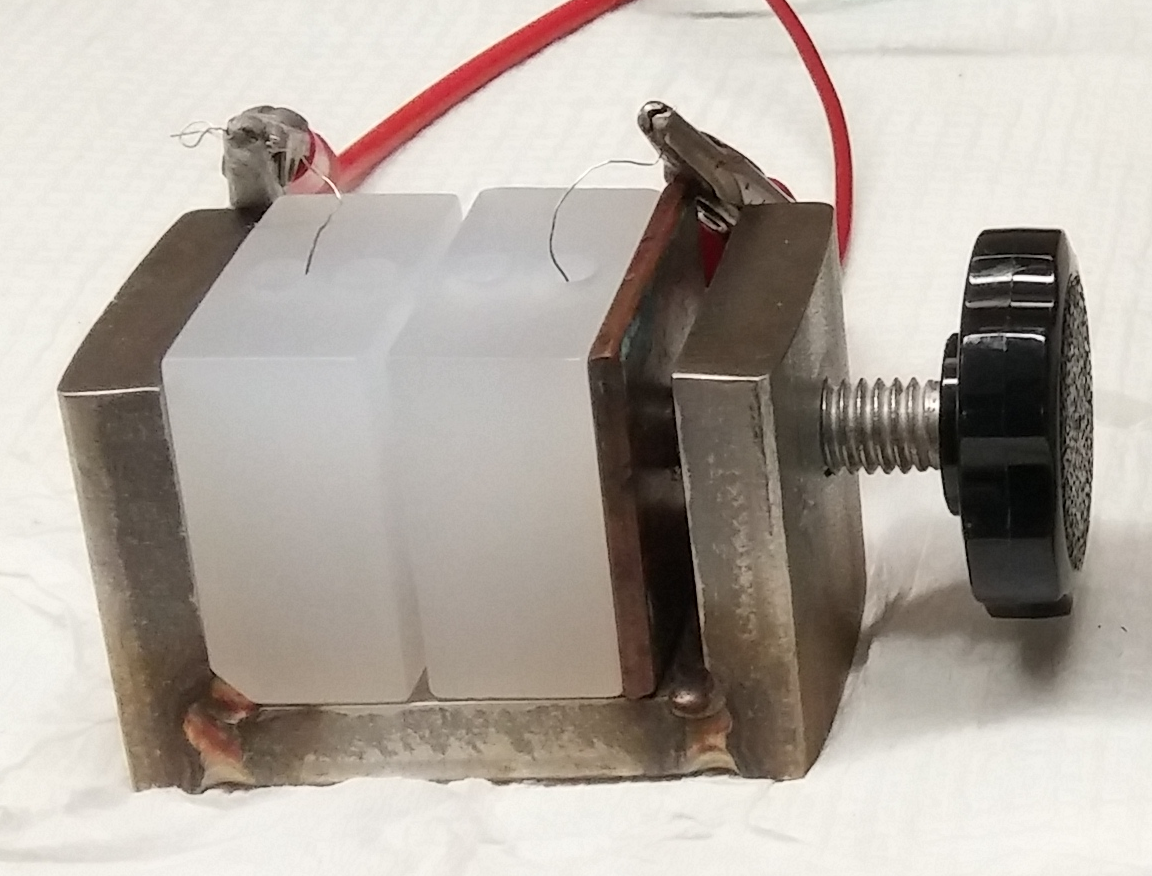
\includegraphics[width=7cm]{photo/conductivitycell.png}}
		%\put(100,0){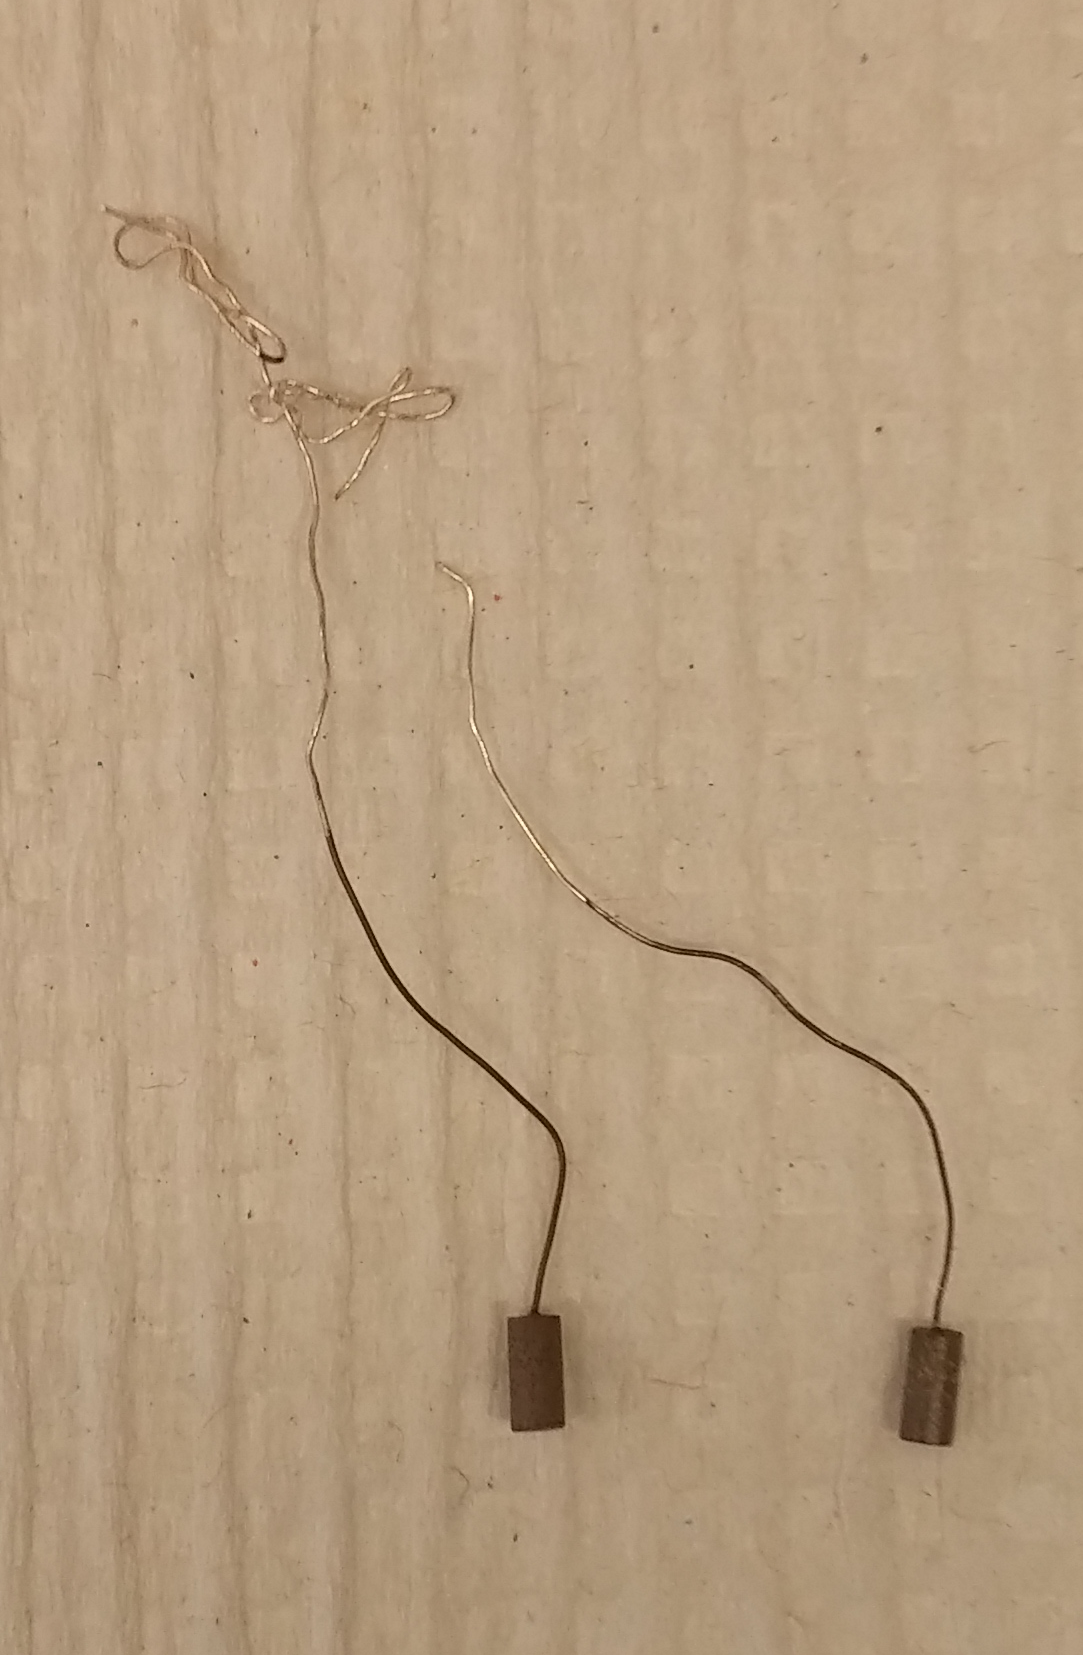
\includegraphics[width=2cm]{photo/electrodes.png}}
		%\put(10,-20){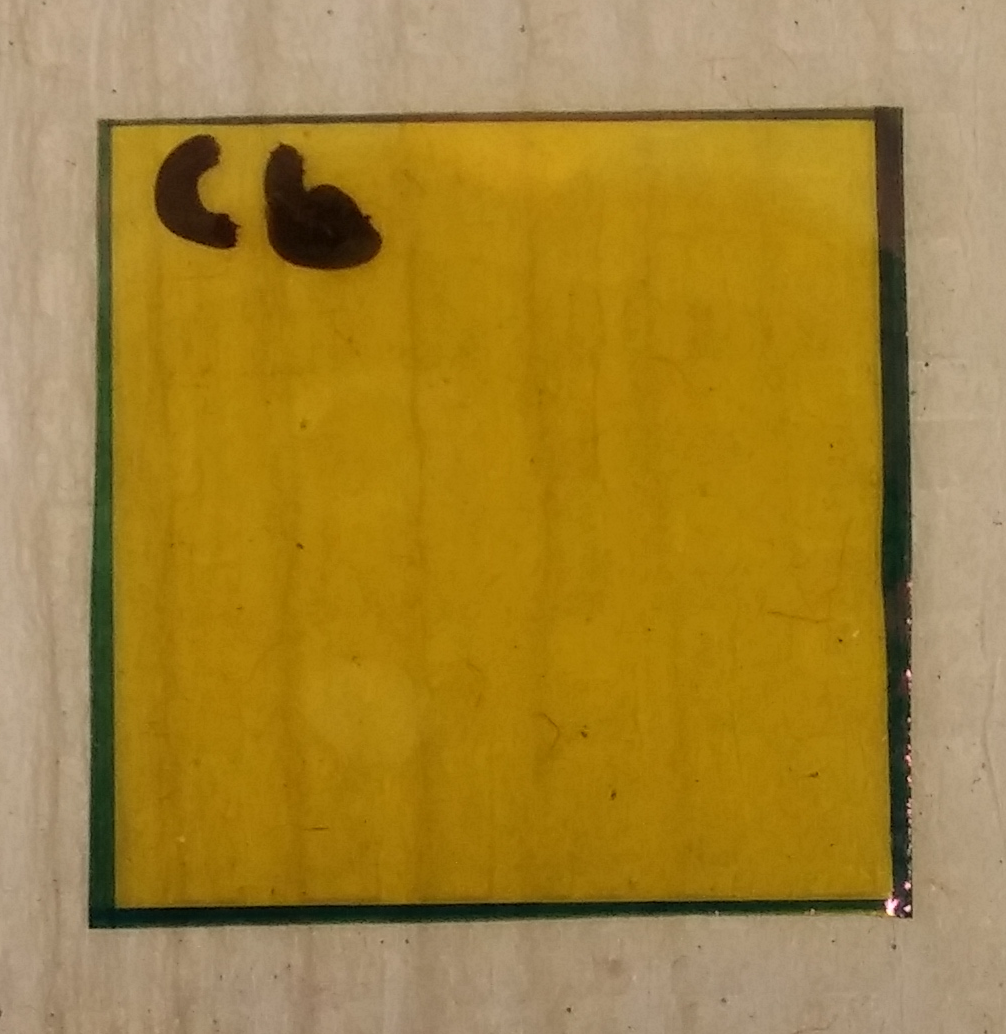
\includegraphics[width=2cm]{photo/membrane.png}}
		%\put(30,-80){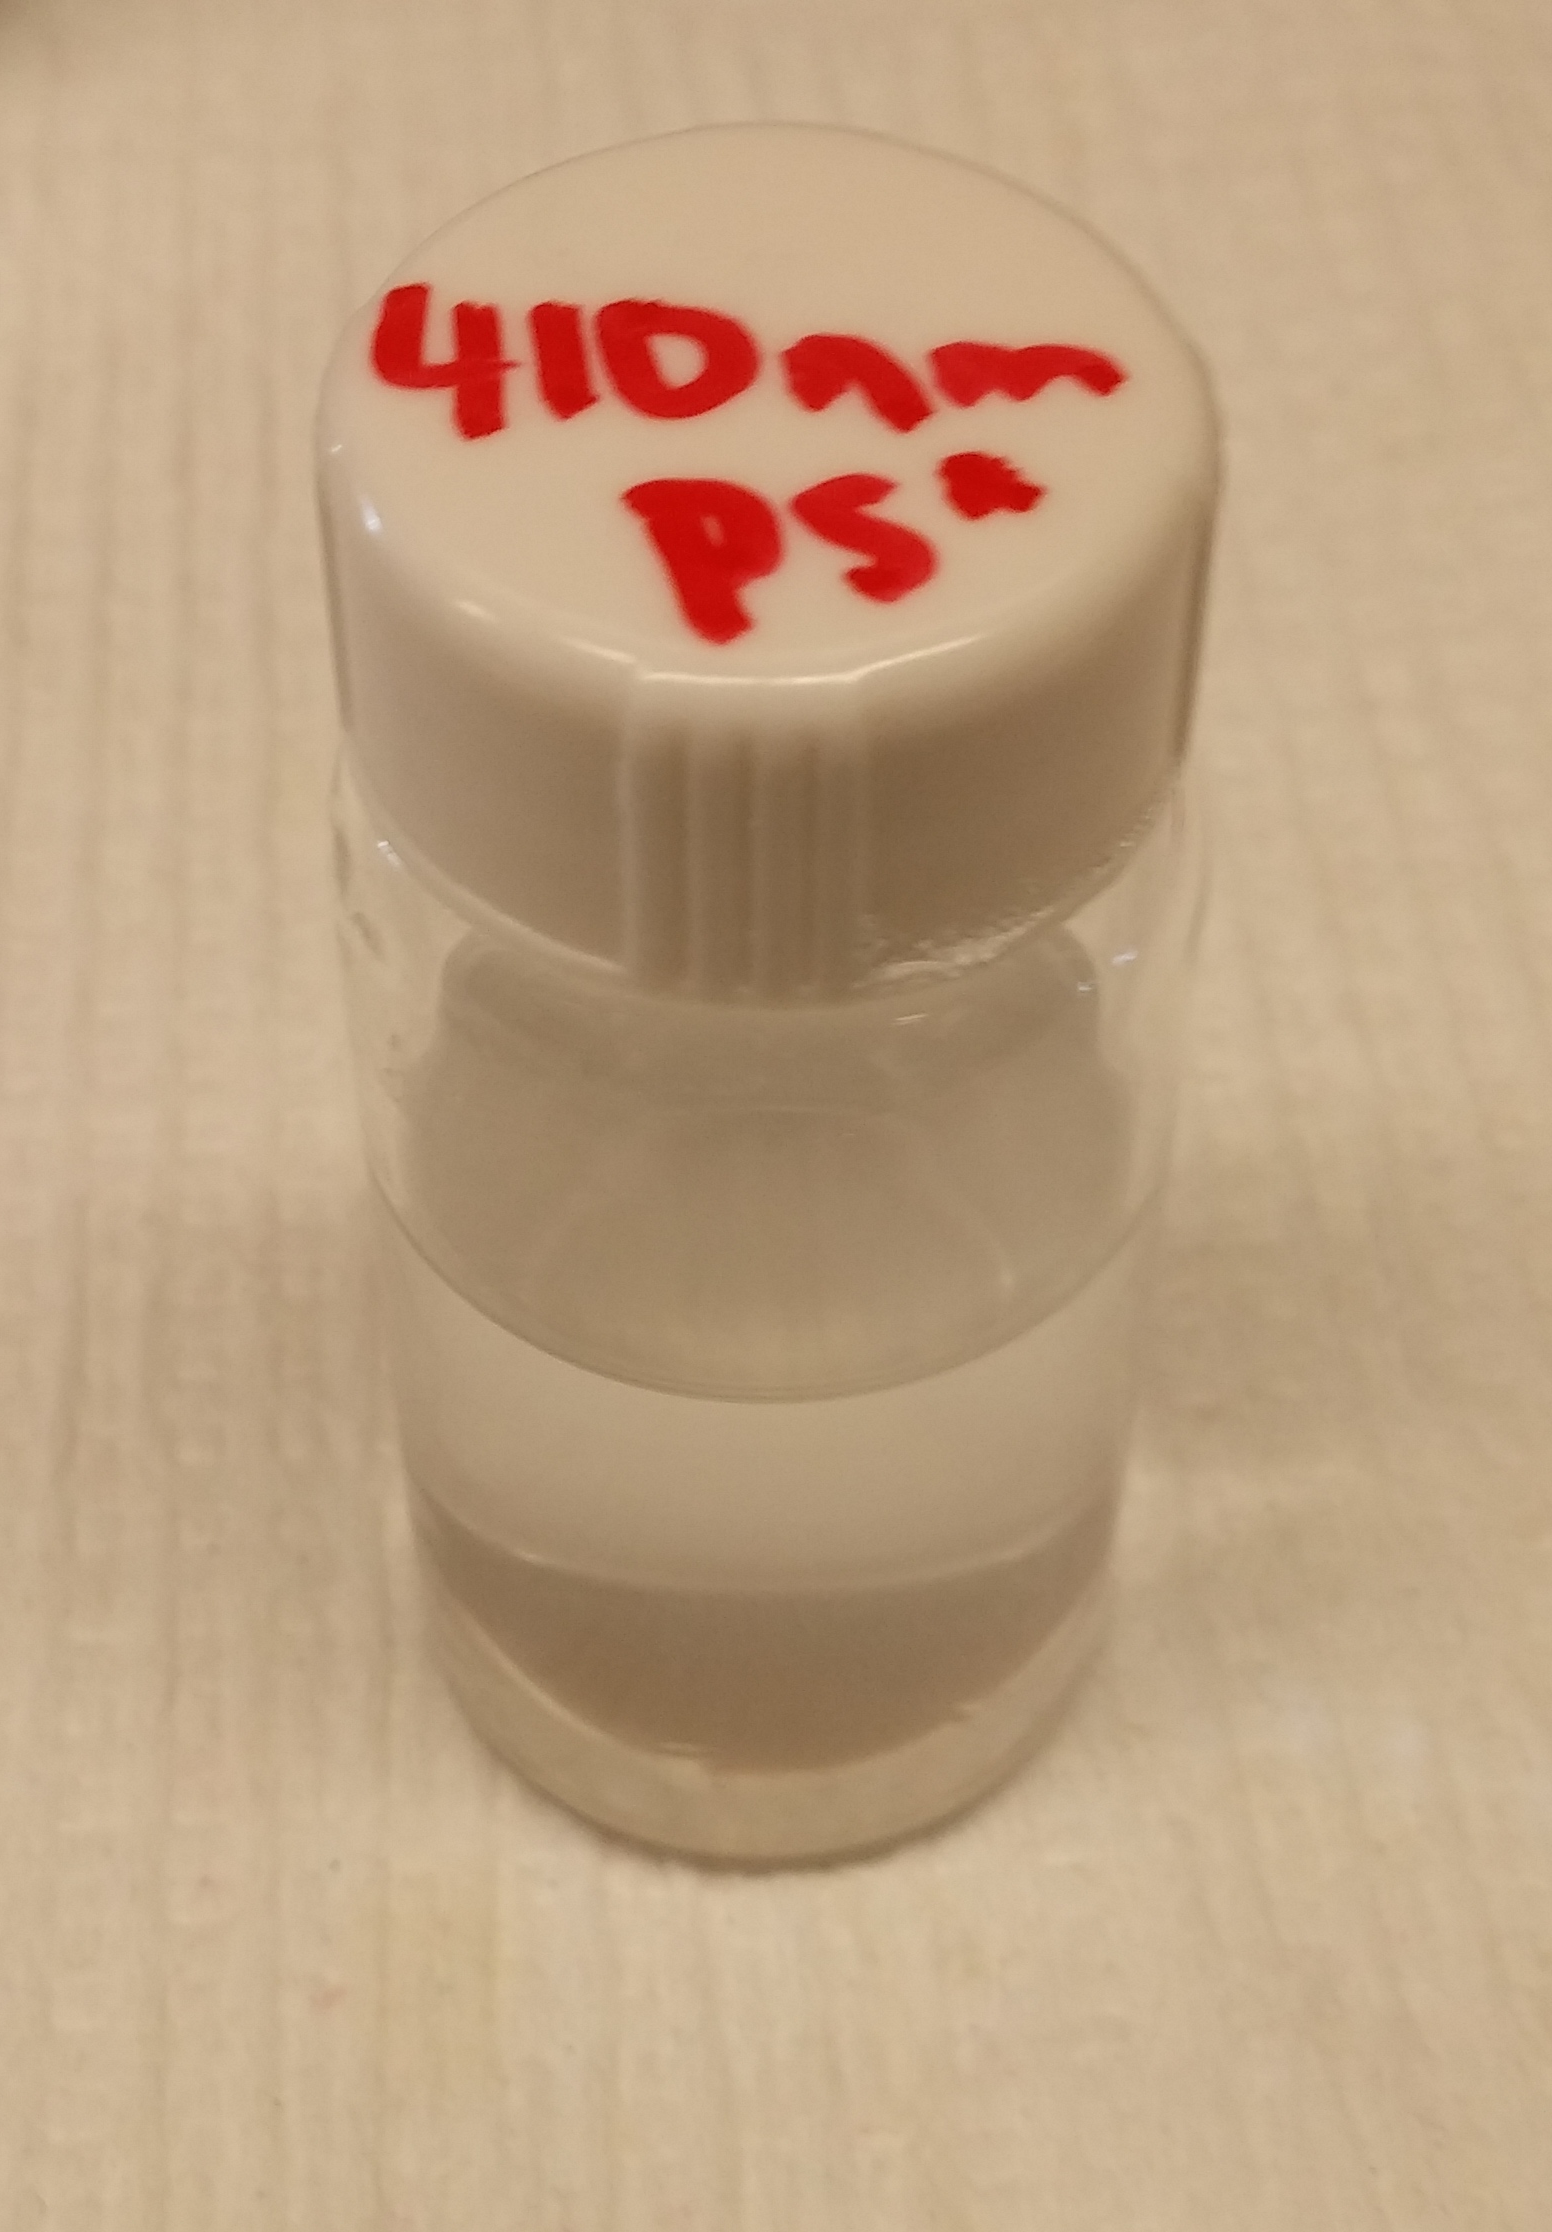
\includegraphics[width=2cm]{photo/solution.png}}
	%\end{picture}
% 	{\centering 
% 		\vspace{0.35cm}
% 		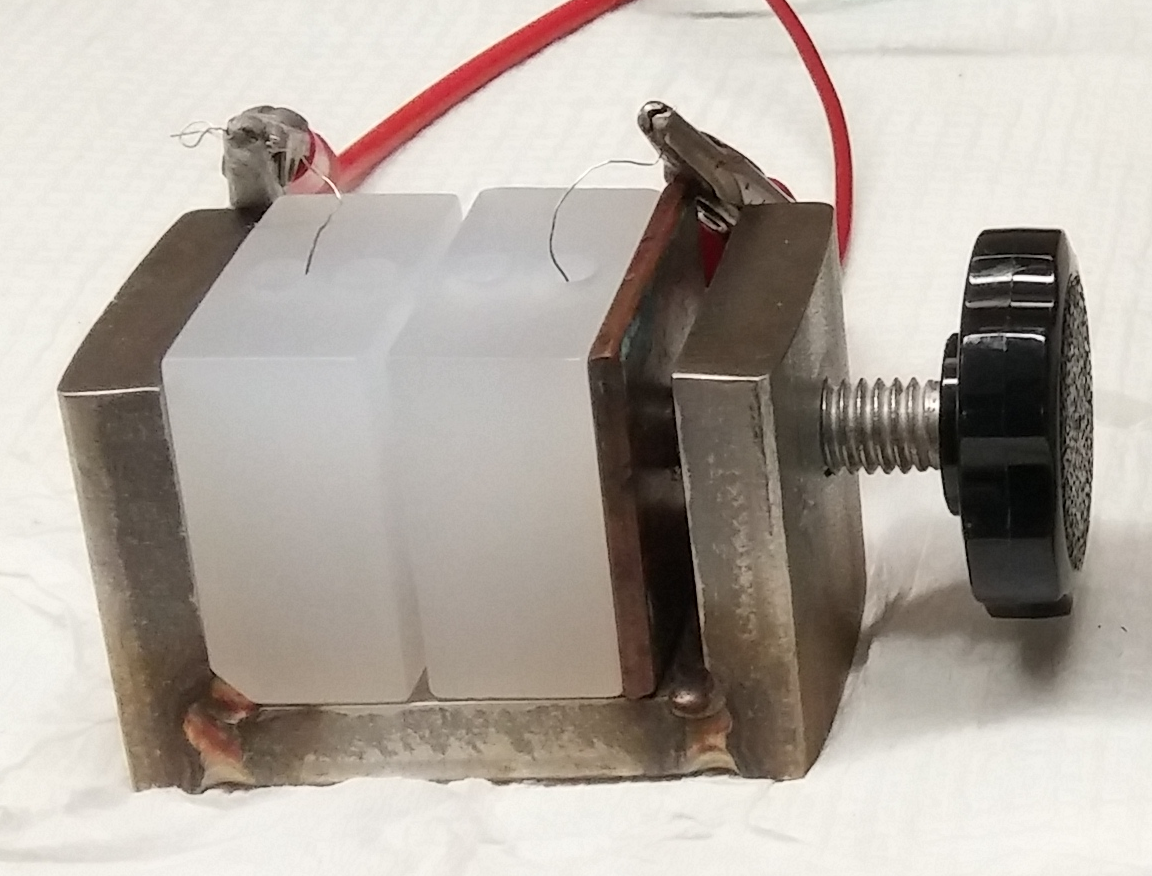
\includegraphics[width=9cm]{photo/conductivitycell.png}
% 		\newline
% 		\vspace{.35cm}
% 		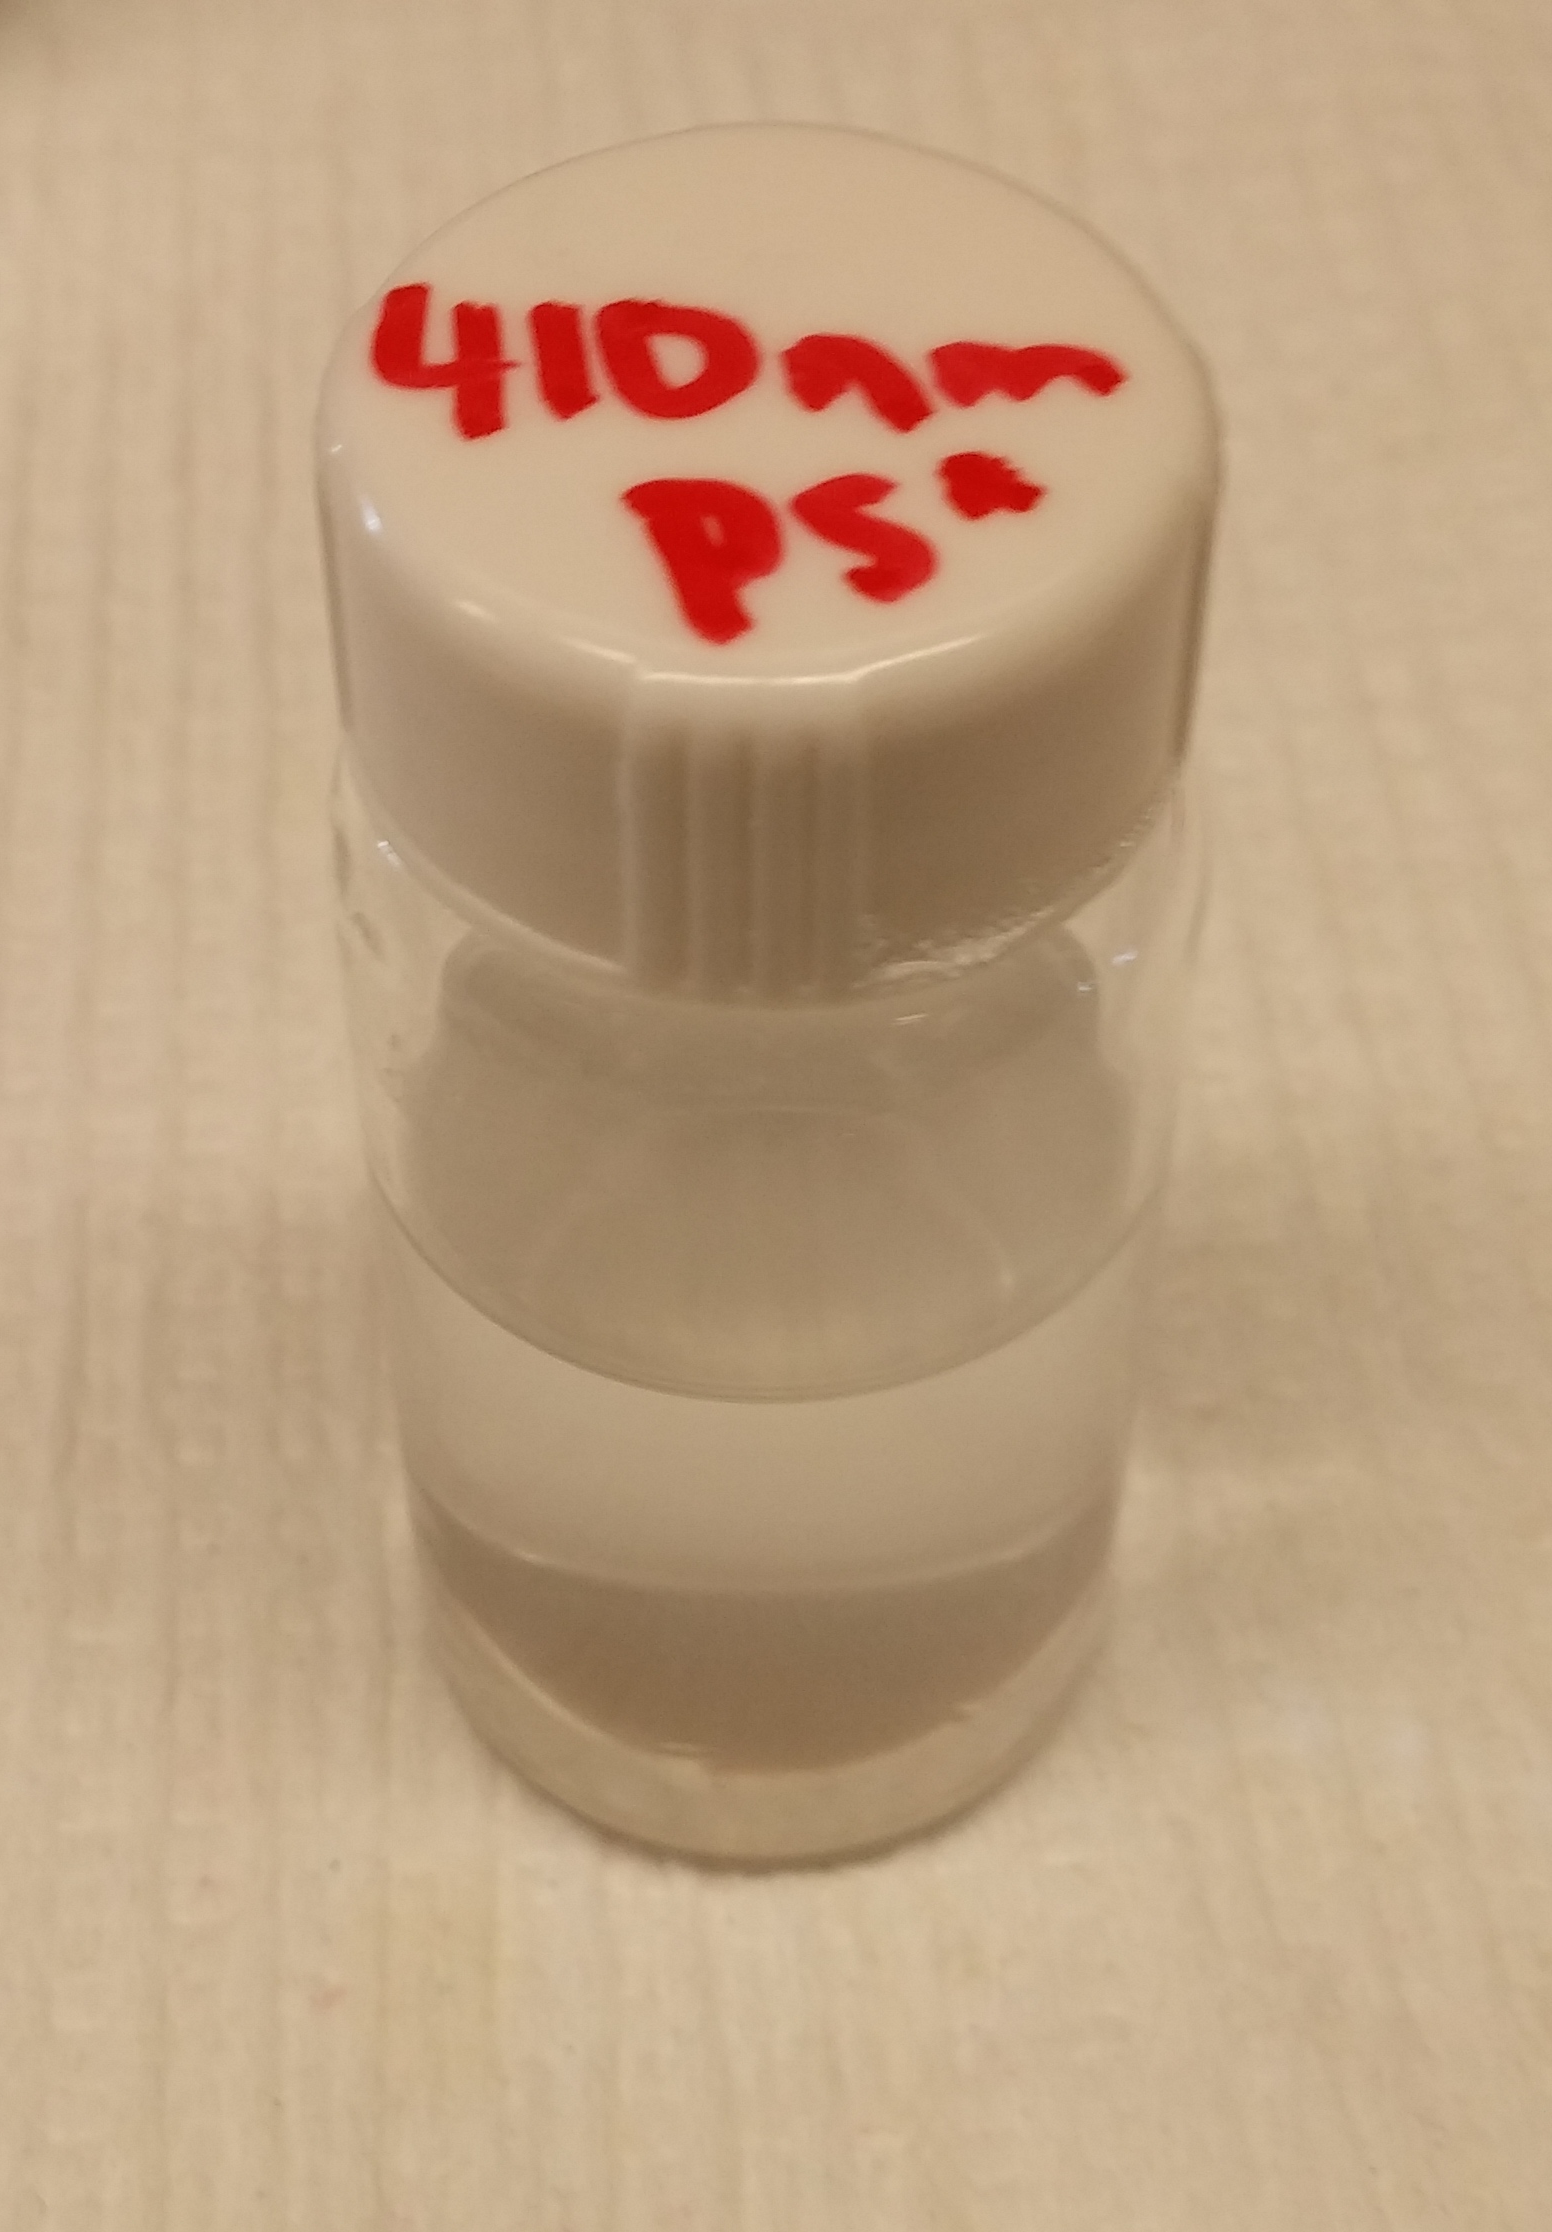
\includegraphics[width=1.5cm]{photo/solution.png}
% 		\hspace{1cm}
% 		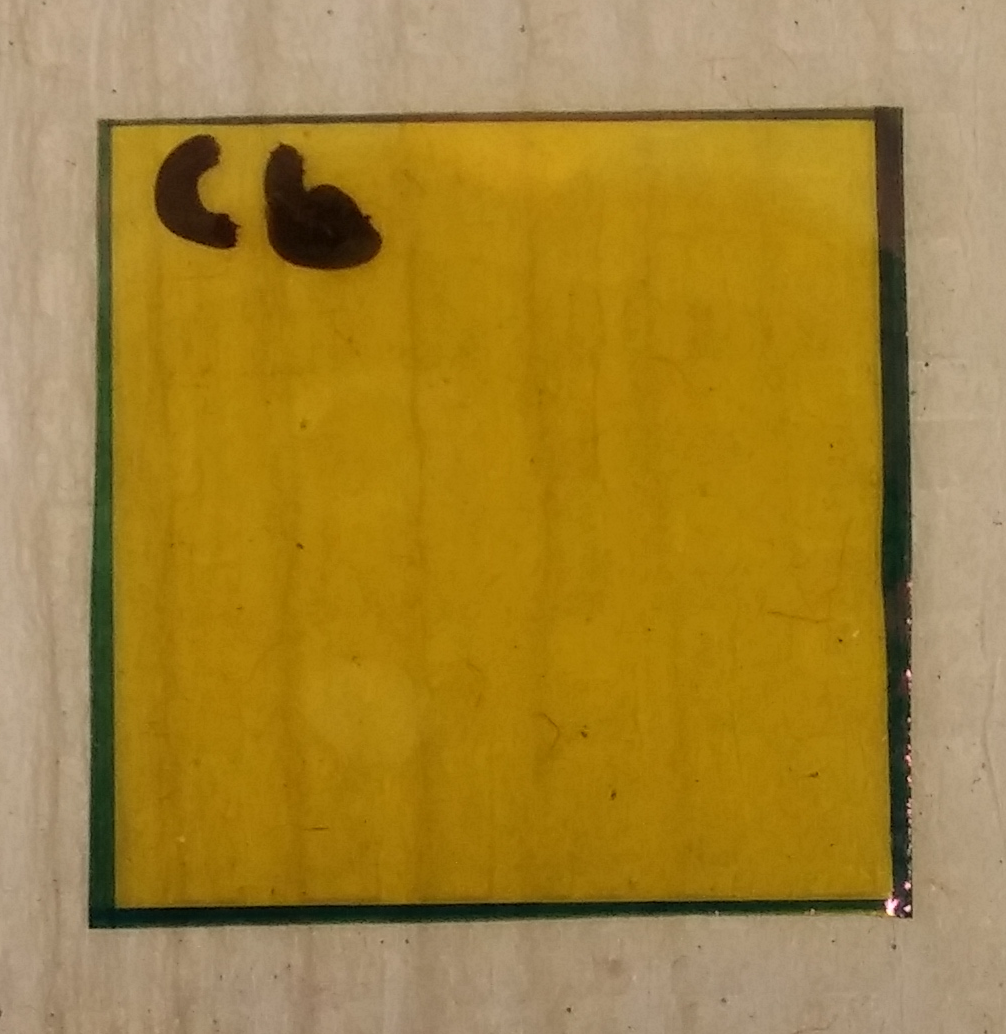
\includegraphics[width=2cm]{photo/membrane.png}
% 		\hspace{1cm}
% 		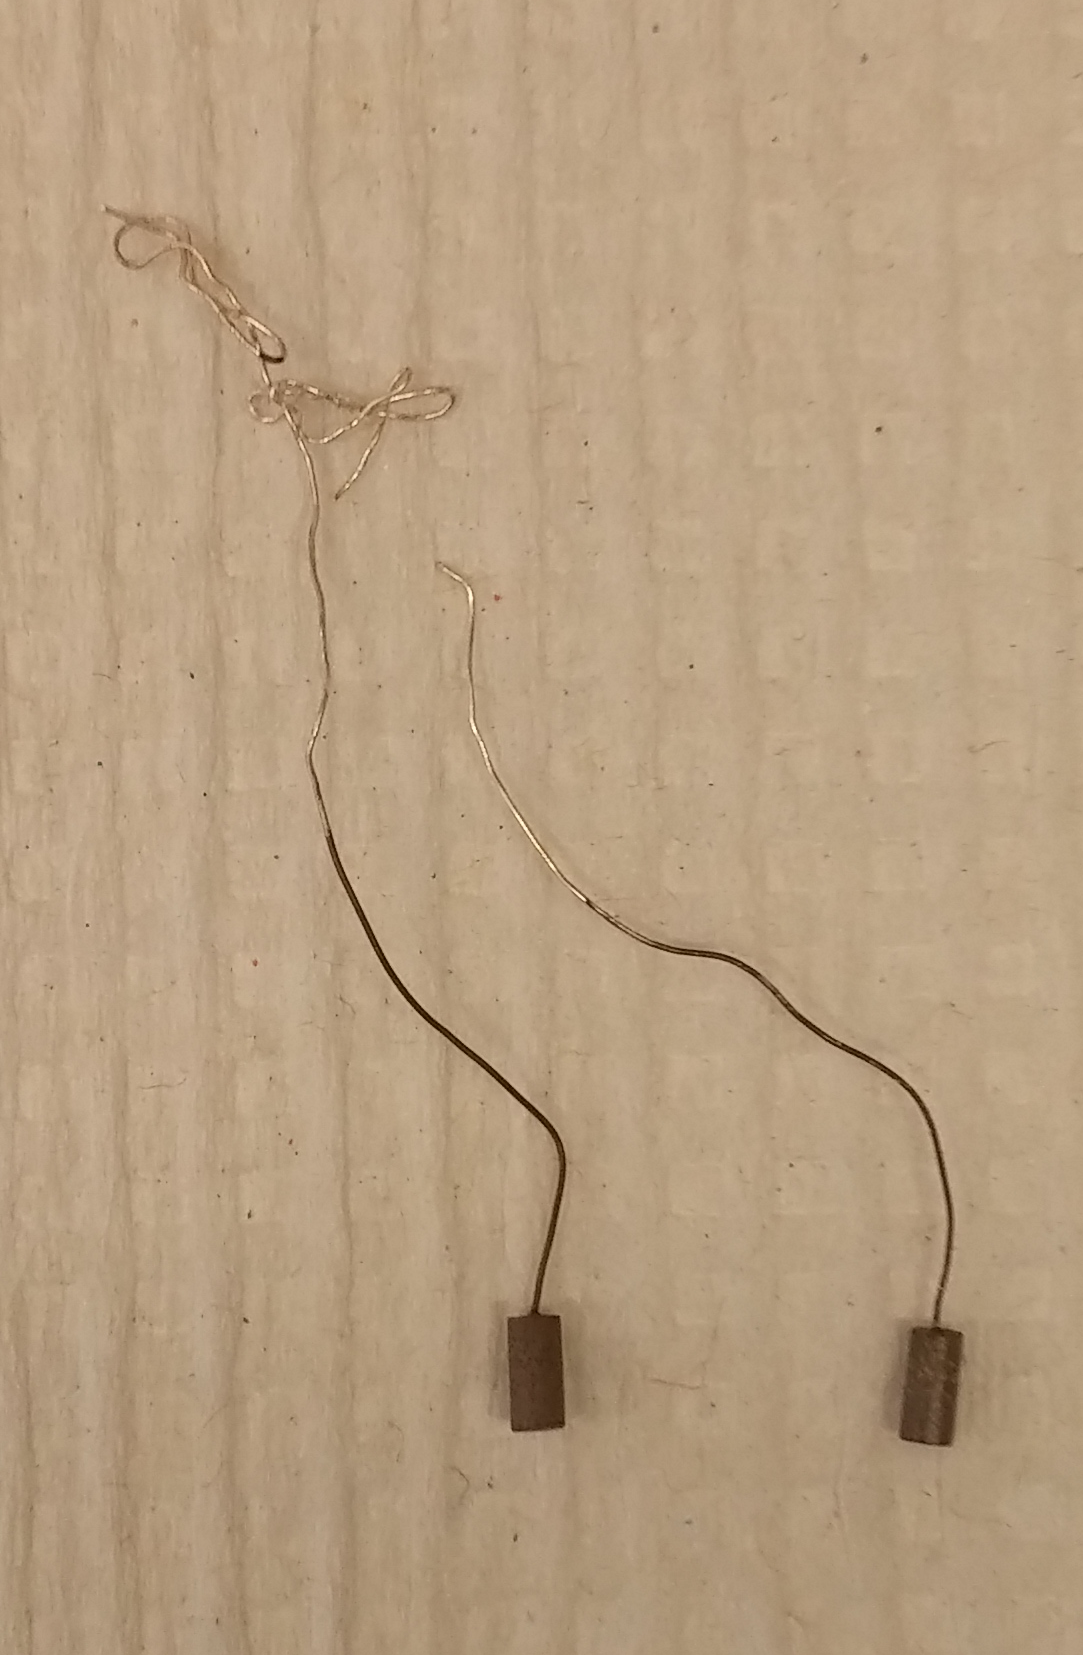
\includegraphics[width=1.5cm]{photo/electrodes.png}
% 		\hspace{1cm}
% 		\par
% 	}


	\begin{columns}[t]
		\begin{column}[T]{\paperwidth/5}
			{\centering
				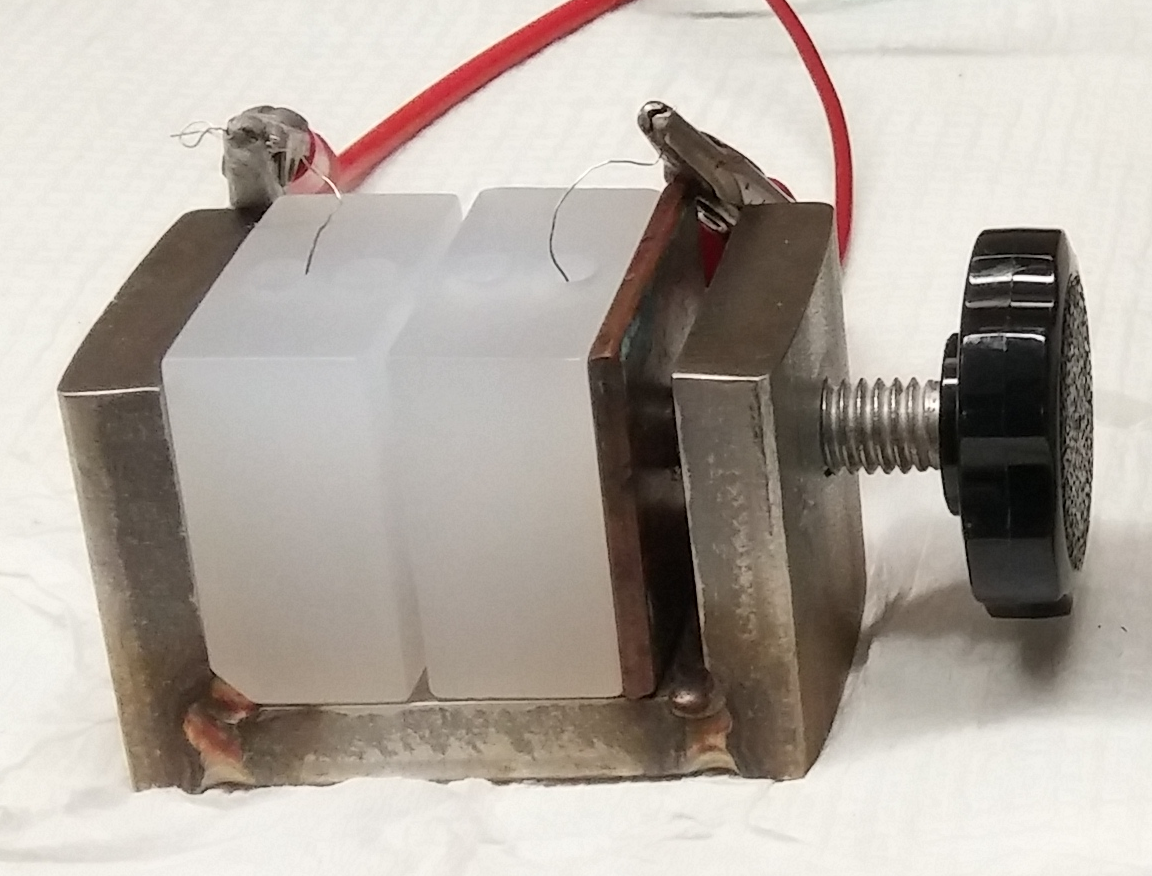
\includegraphics[height=2.25cm]{photo/conductivitycell.png} \\
				{\footnotesize Conductivity cell}
				\par
			}
		\end{column}
		
		
		\begin{column}[T]{\paperwidth/5}
			{\centering
				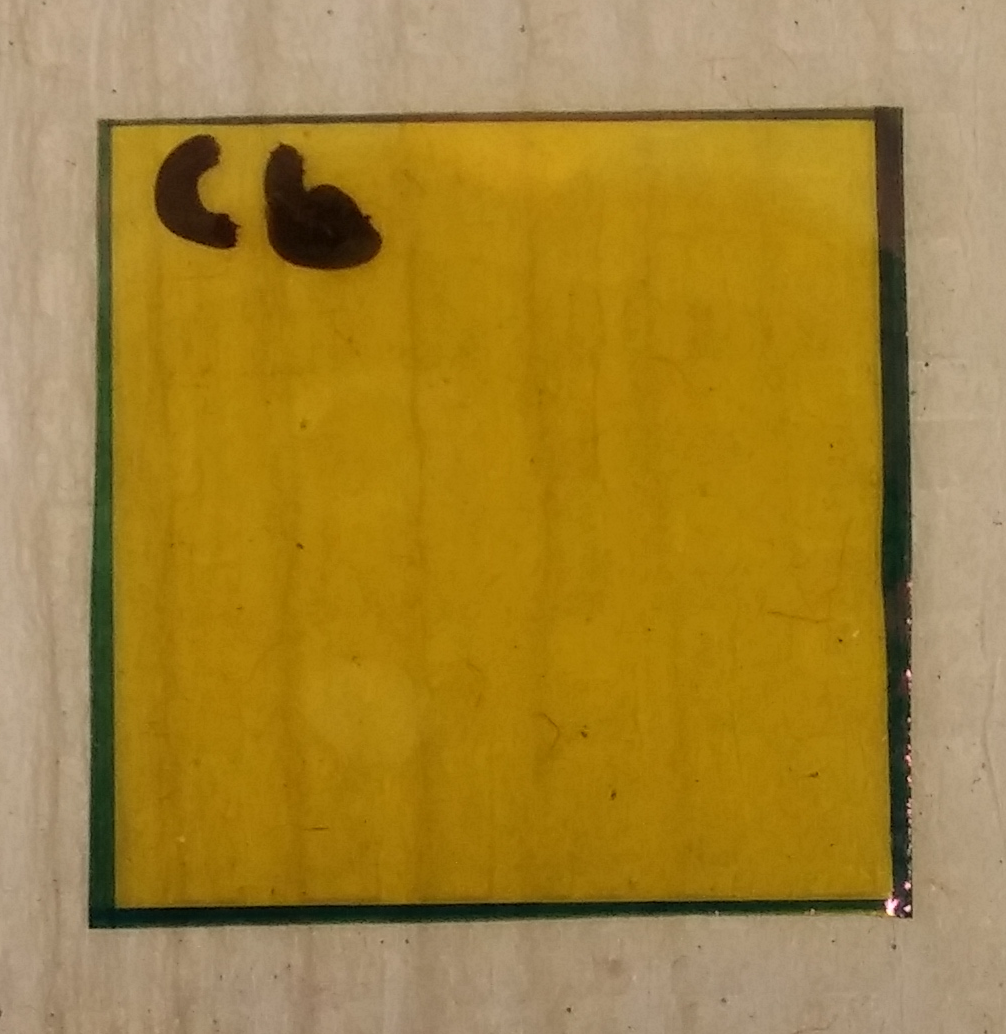
\includegraphics[height=2.25cm]{photo/membrane.png} \\
				{\footnotesize Pore membrane}
				\par
			}
		\end{column}
		
		
		
		\begin{column}[T]{\paperwidth/5}
			{\centering
				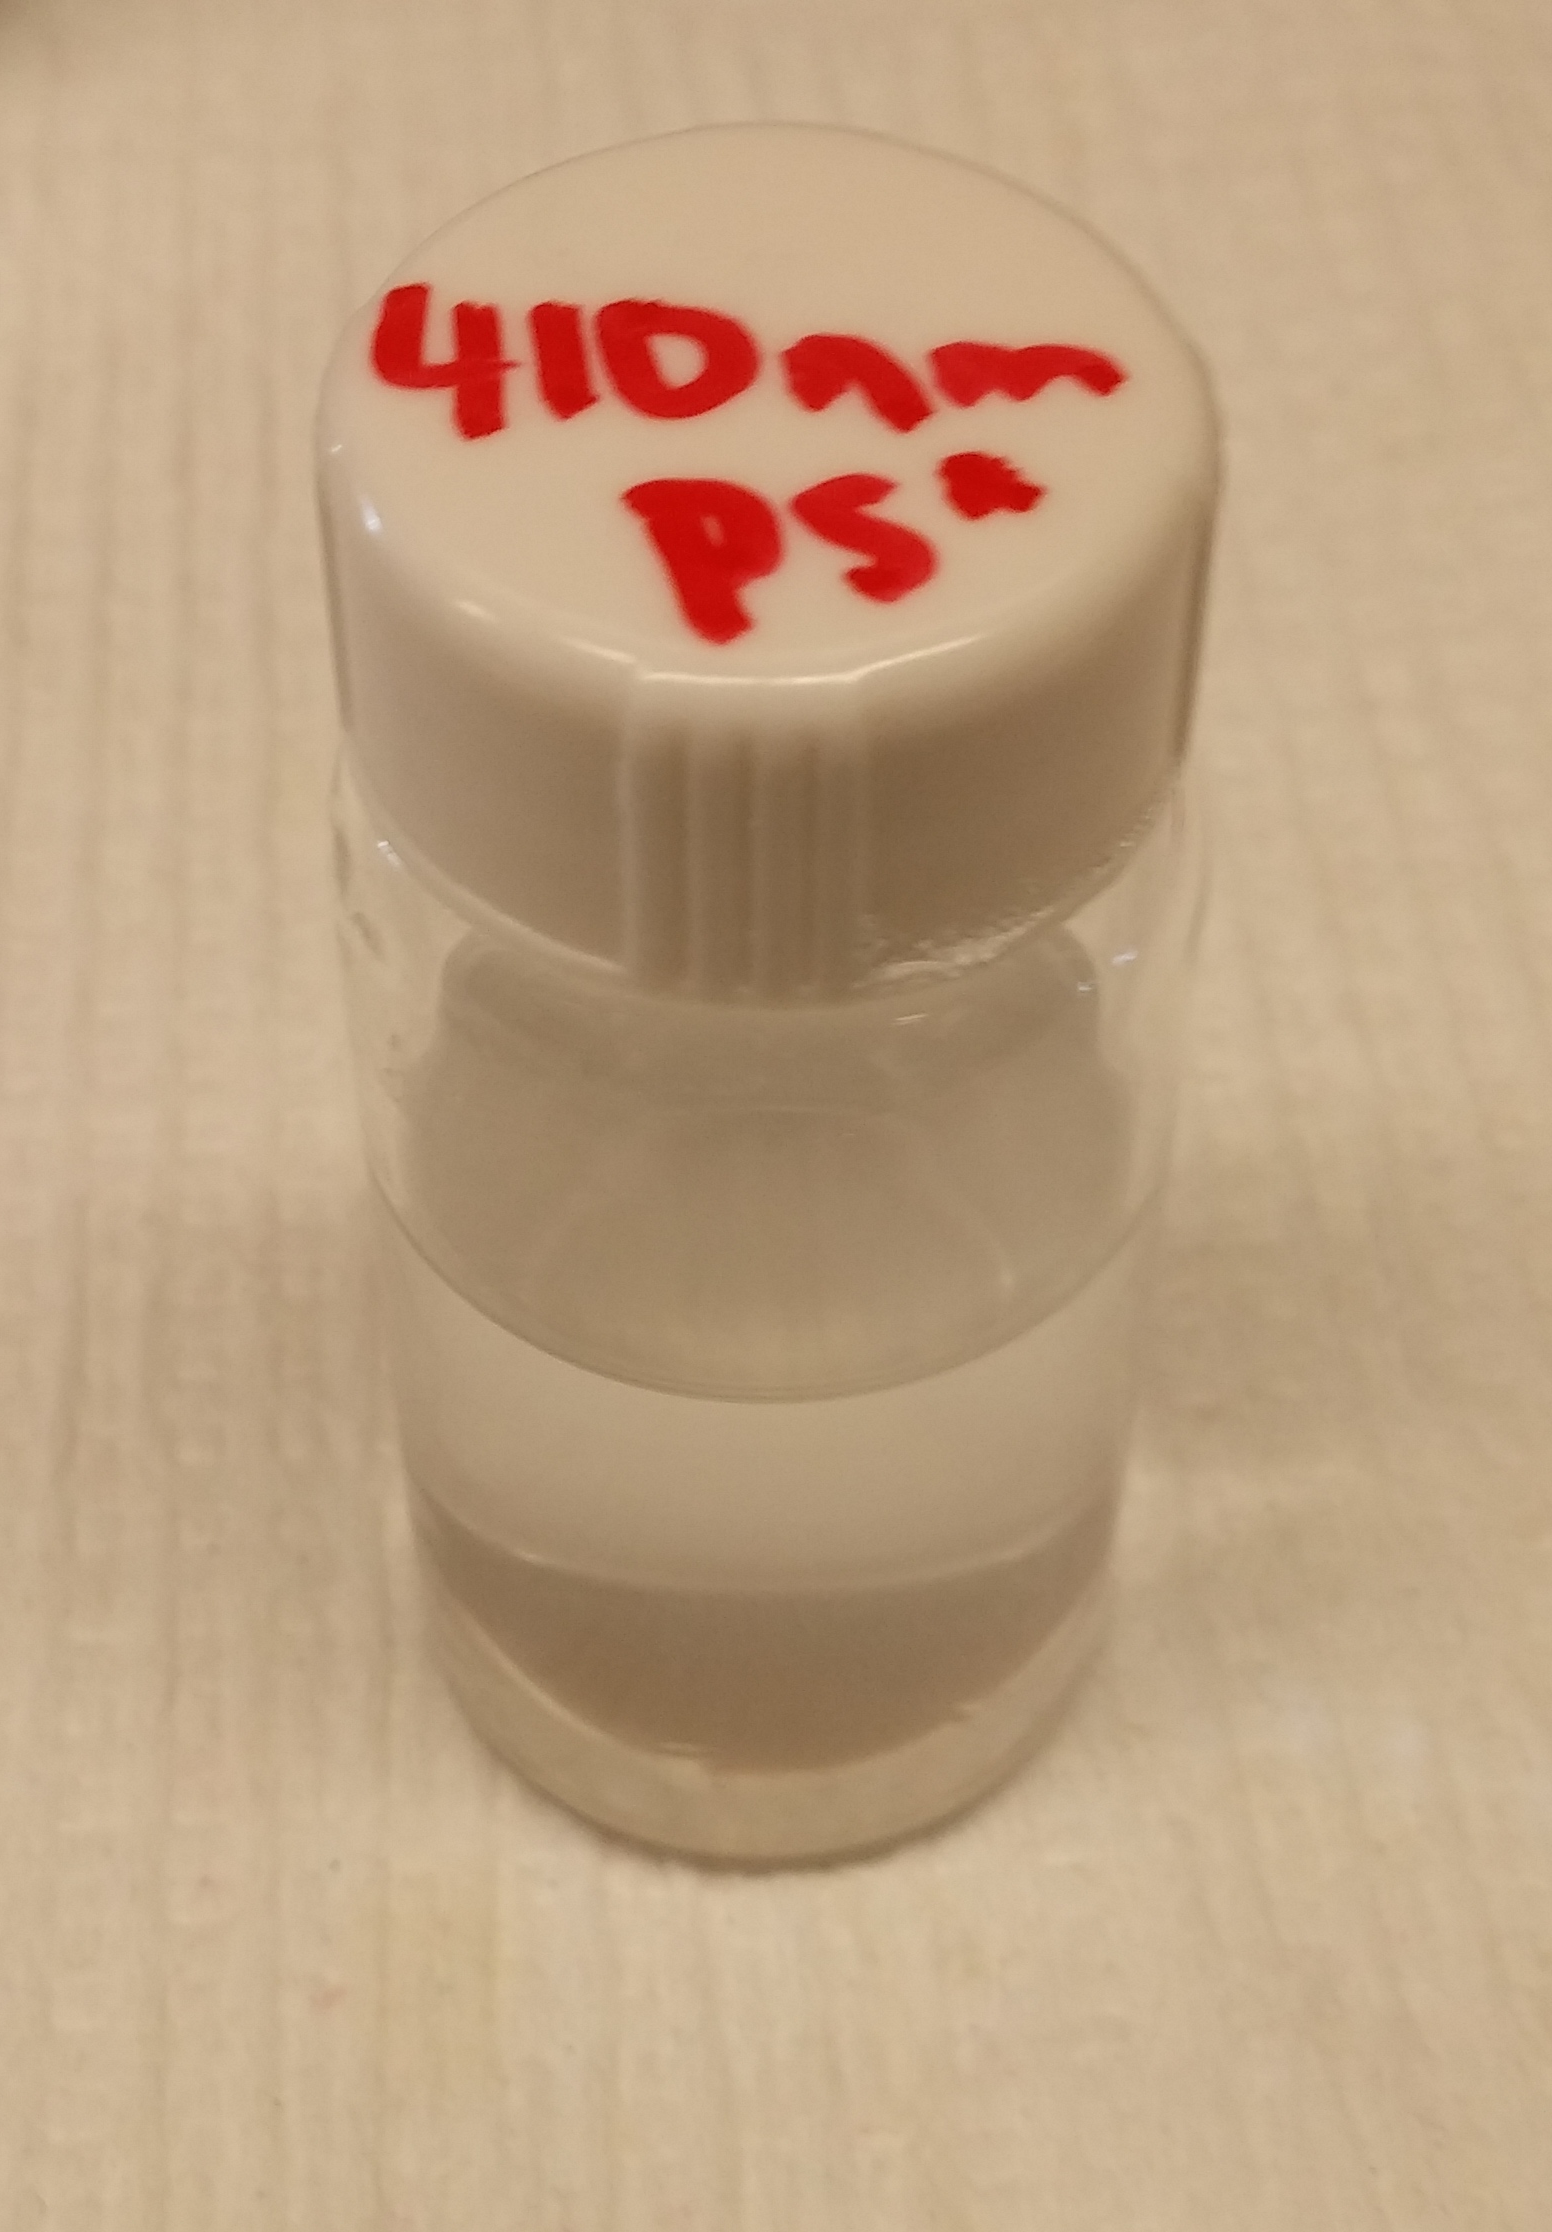
\includegraphics[height=2.25cm]{photo/solution.png} \\
				{\footnotesize Electrolyte}
				\par
			}
		\end{column}

		
		

		
		\begin{column}[T]{\paperwidth/5}
			{\centering
				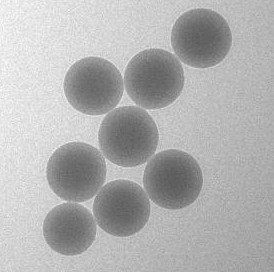
\includegraphics[height=2.25cm]{psbeads} \\
				{\footnotesize Particles}
				\par
			}
		\end{column}

	\end{columns}
	
	\vspace{1cm}
	
	\begin{columns}[t]
		\begin{column}[T]{\paperwidth/5}
			{\centering
				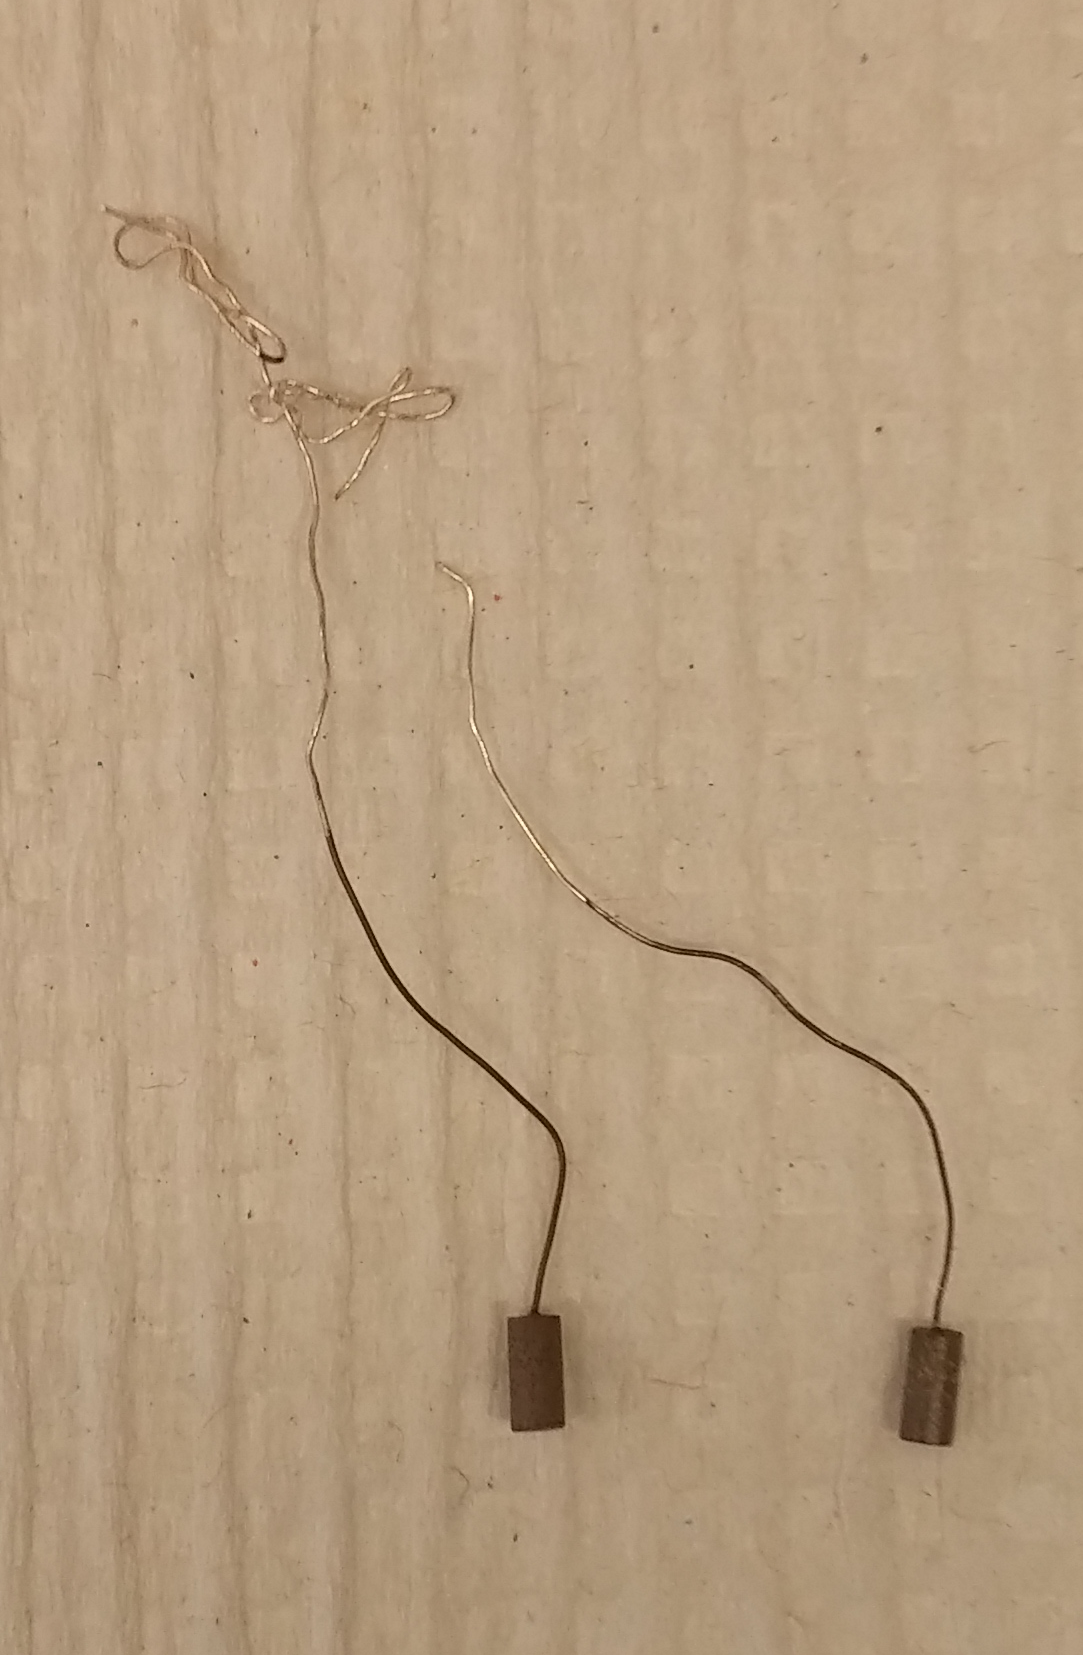
\includegraphics[height=2.25cm]{photo/electrodes.png} \\
				{\footnotesize Ag-AgCl electrodes}
				\par
			}
		\end{column}
		
		
		\begin{column}[T]{.6\paperwidth}
			{\centering
				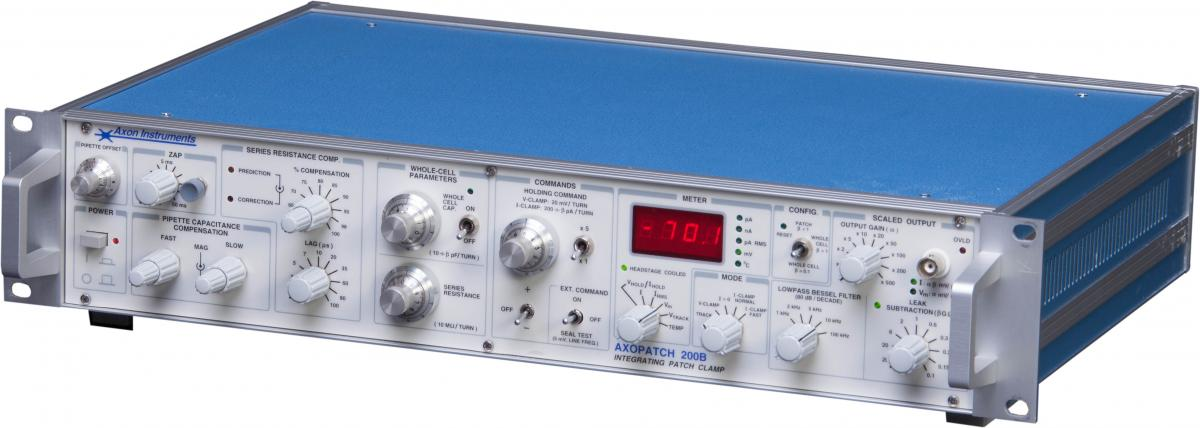
\includegraphics[height=2.25cm]{photo/axon200b} \\
				Voltage amplifier + current recorder
				\par
			}
		\end{column}
	

	\end{columns}




% 	
% 
% 
% 	\begin{center}
% 		\begin{figure}
% 		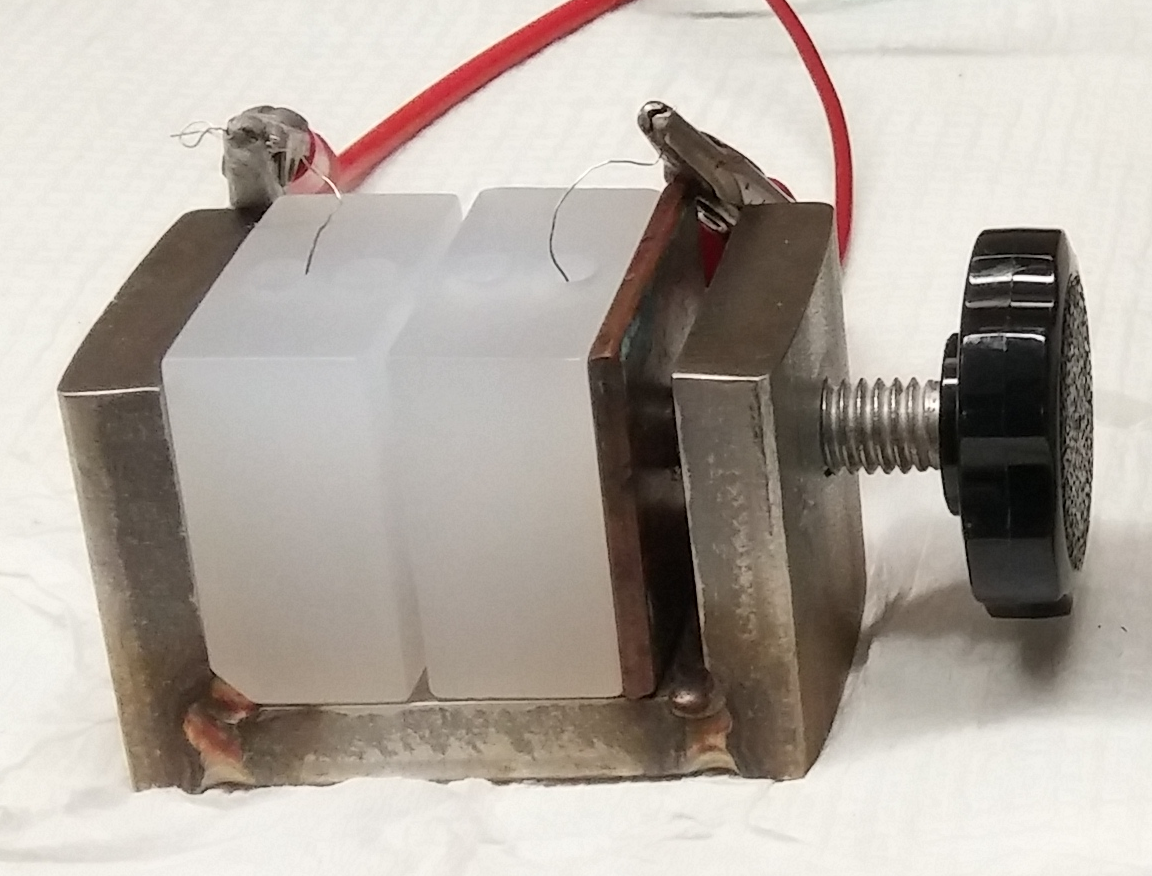
\includegraphics[height=2.25cm]{photo/conductivitycell.png}
% 		\caption{asdf}
% 		\end{figure}
% 		\hspace{.35cm}
%  		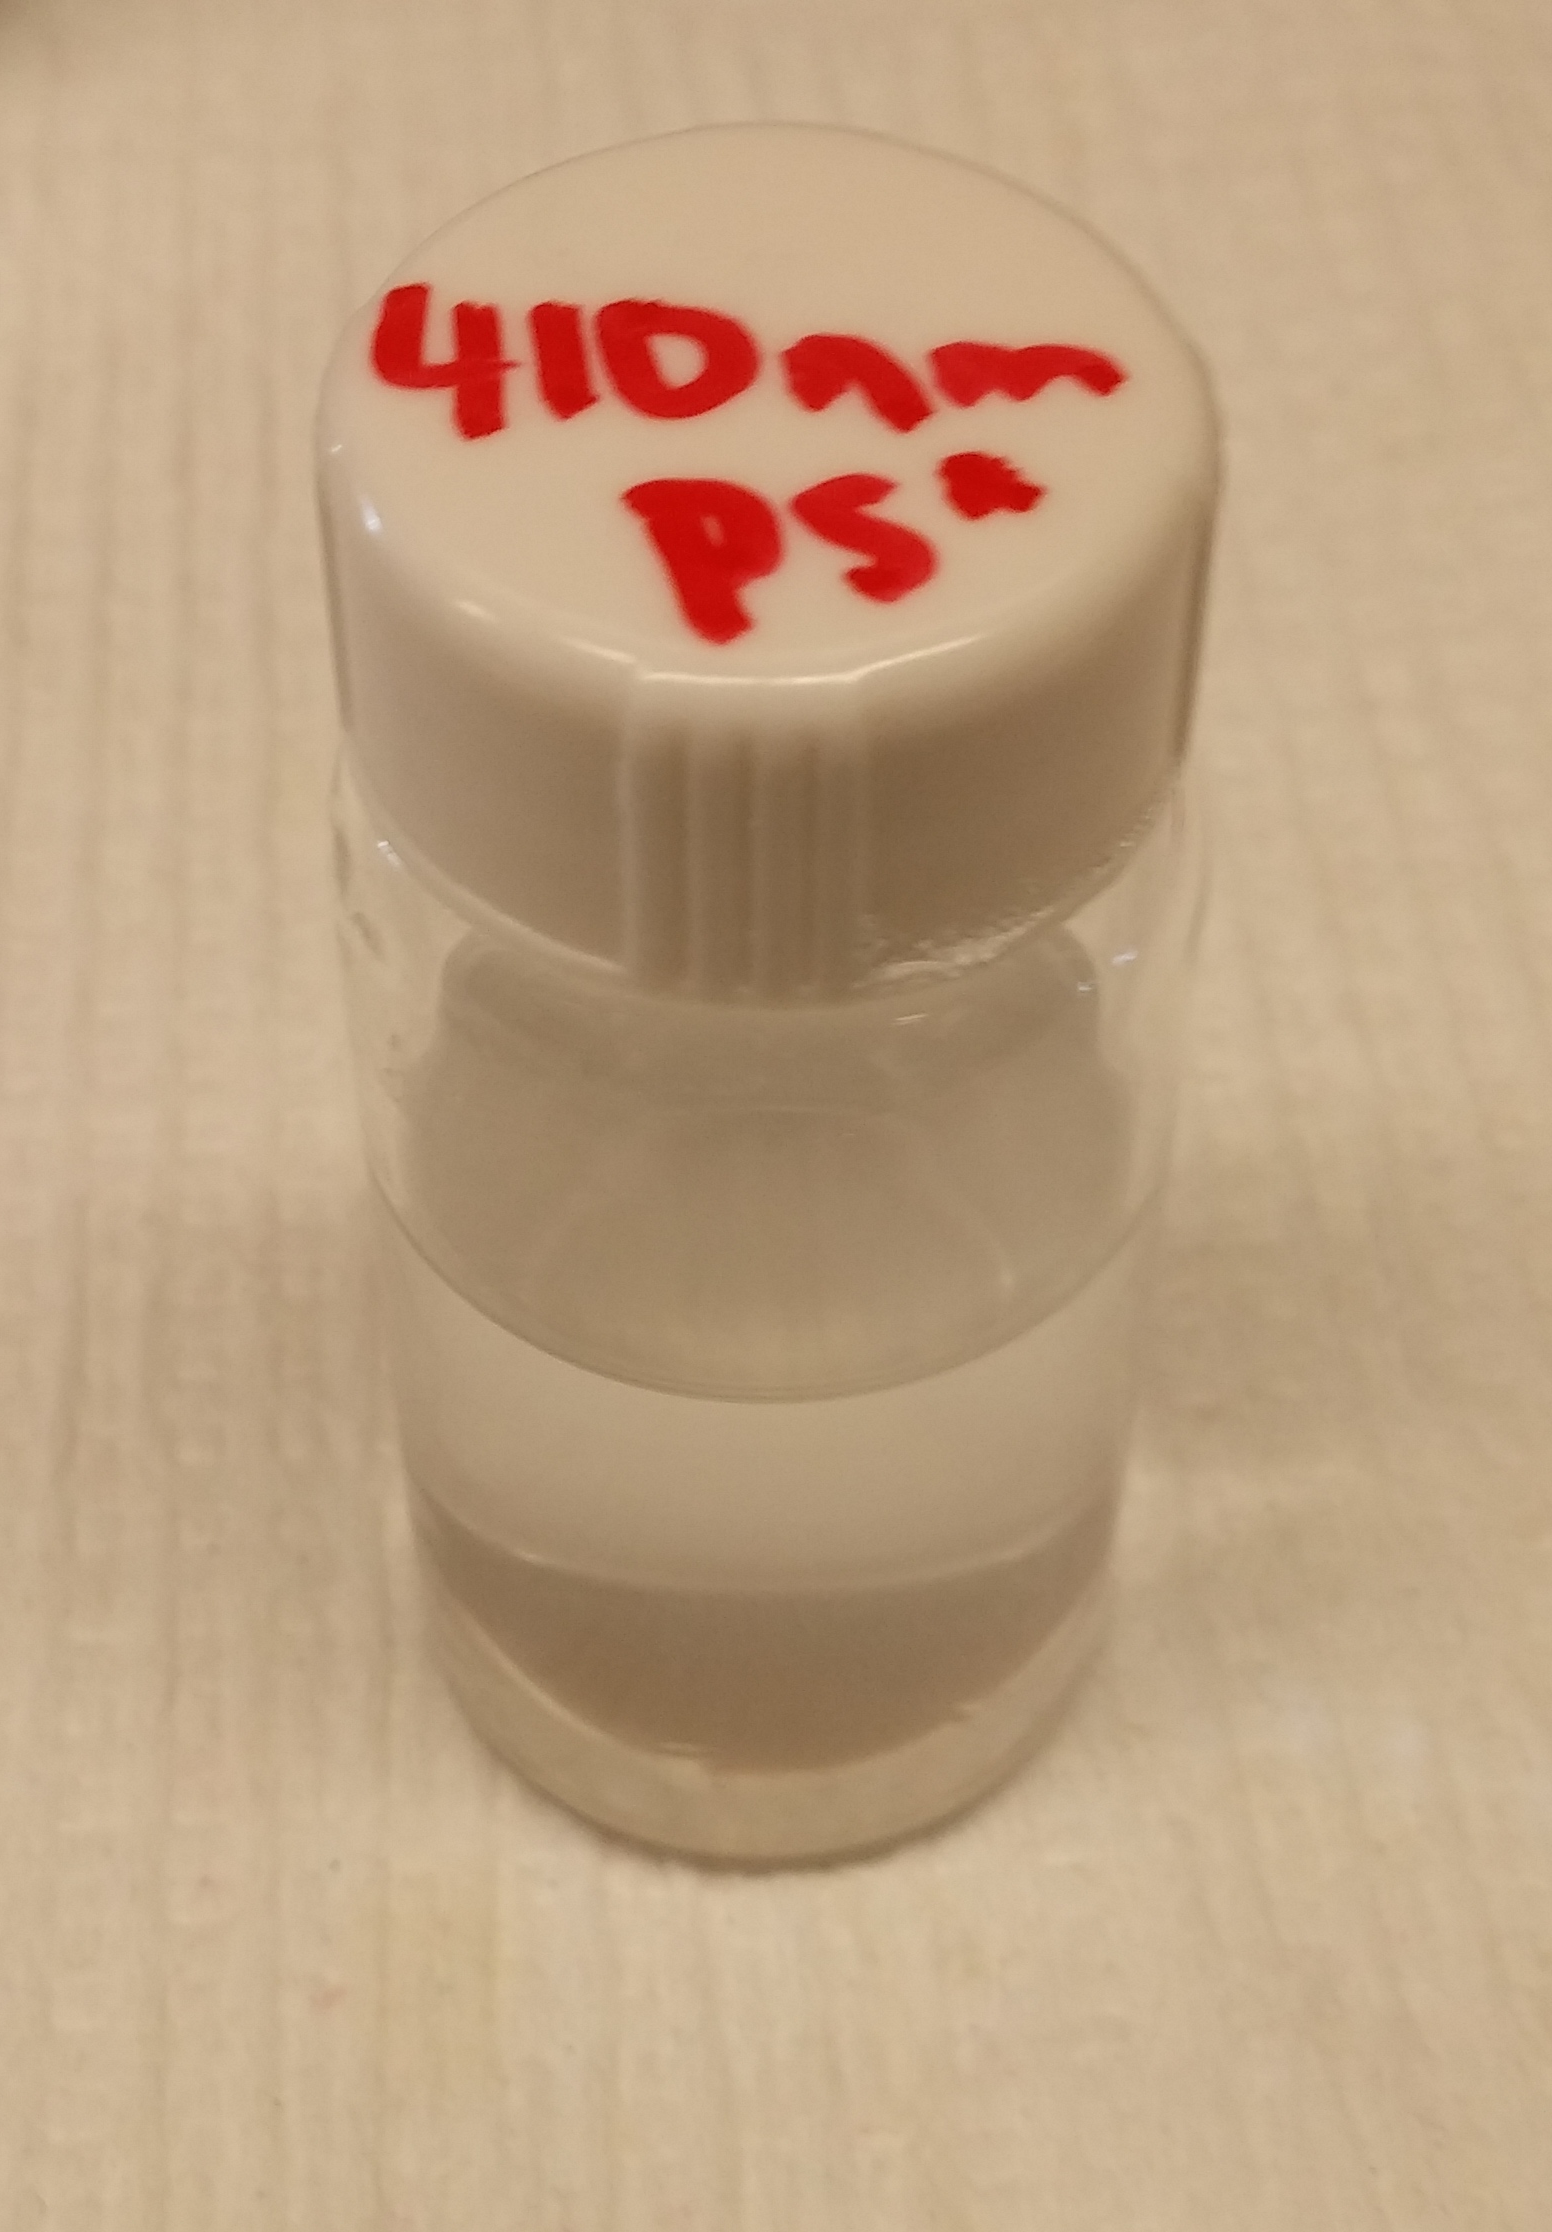
\includegraphics[height=2.25cm]{photo/solution.png}
%  		\hspace{.35cm}
%  		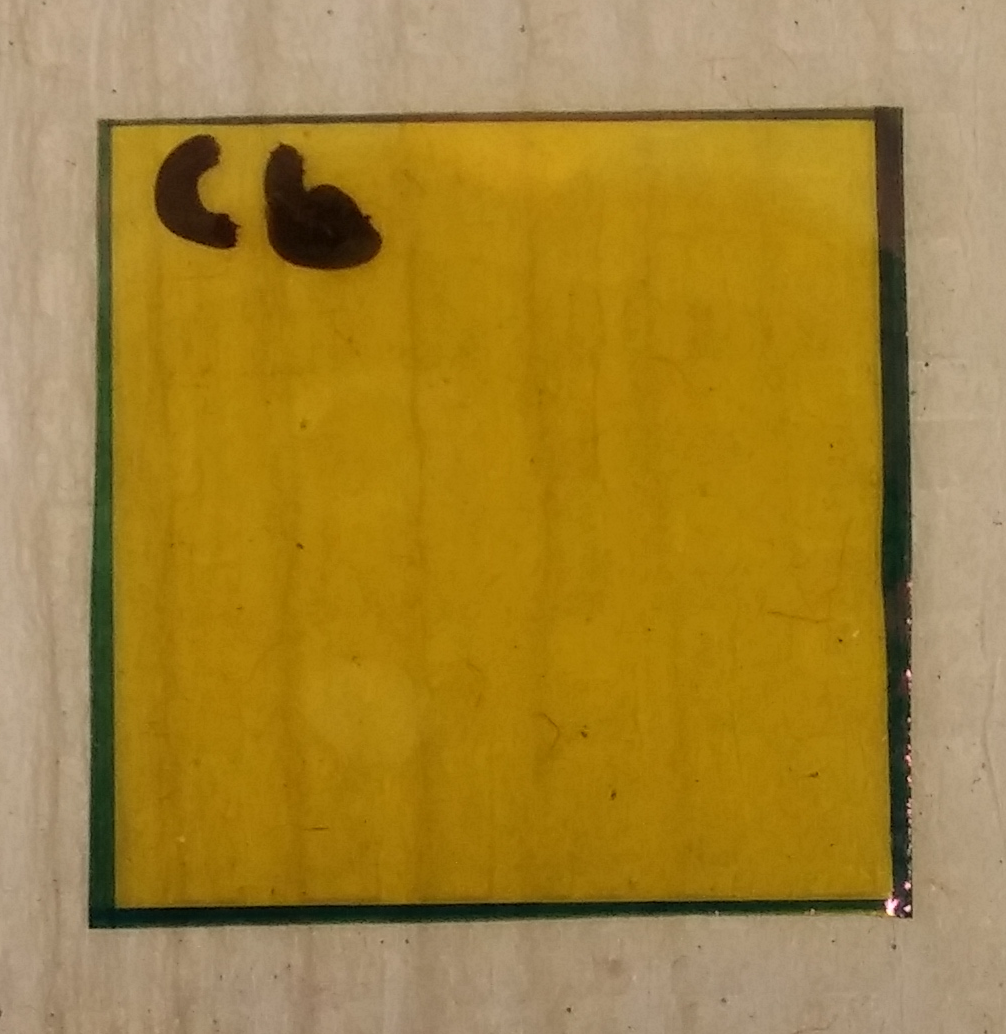
\includegraphics[height=2.25cm]{photo/membrane.png}
%  		\hspace{.35cm}
%  		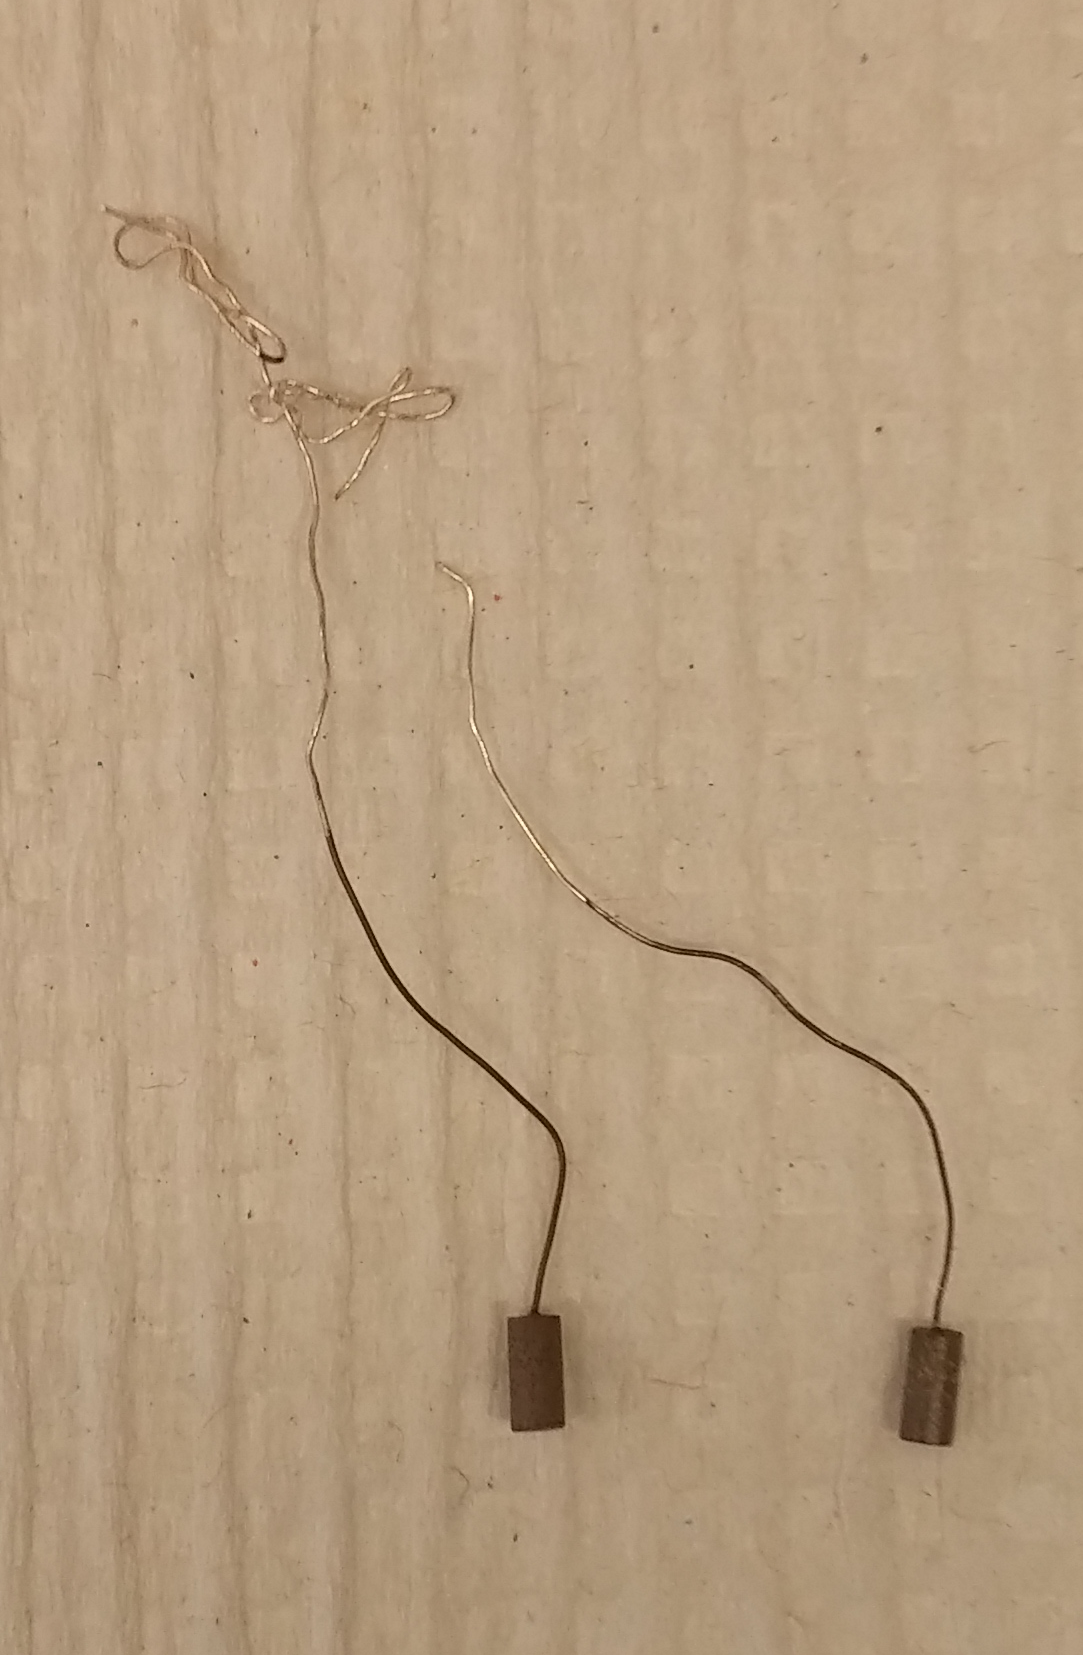
\includegraphics[height=2.25cm]{photo/electrodes.png}
%  		\hspace{.35cm}
% 	\end{center}

\end{frame}

%%%%%%%%%%%%%%%%%%%%%%%%%%%%%%%%%%%%%%%%%%%%%%%%%%%%%%%%%%%%%%%%%%%%%%%%%%%%%%%%%%%%%%%%%%%%%%%%%%%%%%%%%%%%%%%%%%%%%%%%%%%%
% Resistive pulse background---electrostatic boundary conditions
%%%%%%%%%%%%%%%%%%%%%%%%%%%%%%%%%%%%%%%%%%%%%%%%%%%%%%%%%%%%%%%%%%%%%%%%%%%%%%%%%%%%%%%%%%%%%%%%%%%%%%%%%%%%%%%%%%%%%%%%%%%%

\begin{frame}[c]{Resistive pulse sensing}
	{\centering
		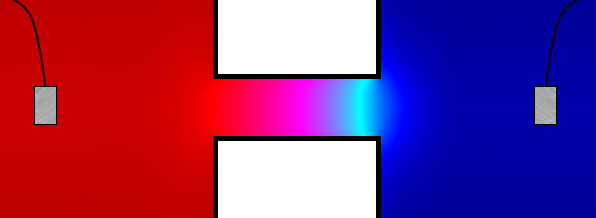
\includegraphics[width=0.9\paperwidth]{comsol/voltage.png}
		\par
	}
\end{frame}

%%%%%%%%%%%%%%%%%%%%%%%%%%%%%%%%%%%%%%%%%%%%%%%%%%%%%%%%%%%%%%%%%%%%%%%%%%%%%%%%%%%%%%%%%%%%%%%%%%%%%%%%%%%%%%%%%%%%%%%%%%%%
% Resistive pulse background---electrostatic boundary conditions
%%%%%%%%%%%%%%%%%%%%%%%%%%%%%%%%%%%%%%%%%%%%%%%%%%%%%%%%%%%%%%%%%%%%%%%%%%%%%%%%%%%%%%%%%%%%%%%%%%%%%%%%%%%%%%%%%%%%%%%%%%%%

\begin{frame}[c]{Resistive pulse sensing---electrostatic boundary conditions}
	{\centering
		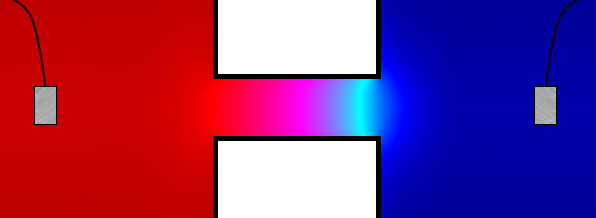
\includegraphics[width=0.9\paperwidth]{comsol/voltage.png}
		\par
	}
\end{frame}


%%%%%%%%%%%%%%%%%%%%%%%%%%%%%%%%%%%%%%%%%%%%%%%%%%%%%%%%%%%%%%%%%%%%%%%%%%%%%%%%%%%%%%%%%%%%%%%%%%%%%%%%%%%%%%%%%%%%%%%%%%%%
% Resistive pulse background---ion transport
%%%%%%%%%%%%%%%%%%%%%%%%%%%%%%%%%%%%%%%%%%%%%%%%%%%%%%%%%%%%%%%%%%%%%%%%%%%%%%%%%%%%%%%%%%%%%%%%%%%%%%%%%%%%%%%%%%%%%%%%%%%%

\tikzset{cross/.style={cross out, draw=black, minimum size=2*(#1-\pgflinewidth), inner sep=0pt, outer sep=0pt},
%default radius will be 1pt. 
cross/.default={1pt}}



\begin{frame}[c]{Resistive pulse sensing---ion transport}
	\begin{itemize}
		\item Ion transport is driven by \textbf{diffusion}, \textbf{convection}, and \textbf{electric migration}
		\item \underline{Diffusion}: Average flow of ions from high to low concentration
		\item \underline{Convection}: Ions move with the fluid/solvent
		\item \underline{Electrical migration}: Ions move in electric field
	\end{itemize}
	\only<1>{
		$$ \vec{J}_{i}=\underbrace{z_{i}eD_{i}\nabla c_{i}}_{\mathrm{diffusion}}+\overbrace{z_{i}ec_{i}\vec{u}}^{\mathrm{convection}}+\underbrace{z_{i}ec_{i}\mu_{i}\vec{E}}_{\mathrm{migration}} $$
	}
	\only<2>{
		$$ \vec{J}_{i}=\underbrace{\xcancel{z_{i}eD_{i}\nabla c_{i}}}_{\mathrm{diffusion}}+\overbrace{\xcancel{z_{i}ec_{i}\vec{u}}}^{\mathrm{convection}}+\underbrace{z_{i}ec_{i}\mu_{i}\vec{E}}_{\mathrm{migration}} $$
	}
	
	$$ I=\sum_{i}\iint_{S}\vec{J_{i}}\cdot \hat{n}dS $$
	
	% xs over two terms in equation
	\onslide<2>{
		\begin{tikzpicture}[]
			\draw(300,25) node[cross=10pt,red] {};
			\draw(1,0) node[cross=10pt,red] {};
		\end{tikzpicture}
	}

\end{frame}




%%%%%%%%%%%%%%%%%%%%%%%%%%%%%%%%%%%%%%%%%%%%%%%%%%%%%%%%%%%%%%%%%%%%%%%%%%%%%%%%%%%%%%%%%%%%%%%%%%%%%%%%%%%%%%%%%%%%%%%%%%%%
% Rods title slide
%%%%%%%%%%%%%%%%%%%%%%%%%%%%%%%%%%%%%%%%%%%%%%%%%%%%%%%%%%%%%%%%%%%%%%%%%%%%%%%%%%%%%%%%%%%%%%%%%%%%%%%%%%%%%%%%%%%%%%%%%%%%


\begin{frame}[c]{}
	\begin{center}
		\textbf{Resistive pulse sensing of high-aspect ratio particles}
	\end{center}
\end{frame}




%%%%%%%%%%%%%%%%%%%%%%%%%%%%%%%%%%%%%%%%%%%%%%%%%%%%%%%%%%%%%%%%%%%%%%%%%%%%%%%%%%%%%%%%%%%%%%%%%%%%%%%%%%%%%%%%%%%%%%%%%%%%
% Rods motivation slide
%%%%%%%%%%%%%%%%%%%%%%%%%%%%%%%%%%%%%%%%%%%%%%%%%%%%%%%%%%%%%%%%%%%%%%%%%%%%%%%%%%%%%%%%%%%%%%%%%%%%%%%%%%%%%%%%%%%%%%%%%%%%


\begin{frame}[c]{High-aspect ratio resistive pulse sensing---motivation}
 	\begin{itemize}
 		\item Aspherical particles are ubiquitous in biology---e.g., many viruses and bacteria are approximately rod-shaped
 	\end{itemize}


	\begin{columns}[t]
		\begin{column}[T]{2.5in}
			{\centering
				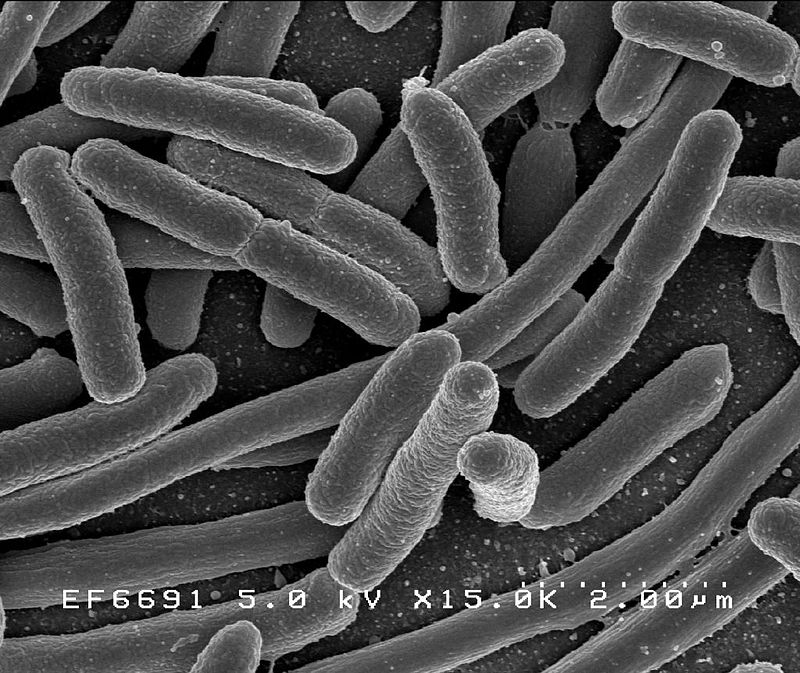
\includegraphics[height=2.25cm]{ecoli} \\
				e. coli \\
				$L\sim \SI{2}{\mu m}$ \\
				\par
			}
		\end{column}
		
		
		\begin{column}[T]{2.5in}
			{\centering
				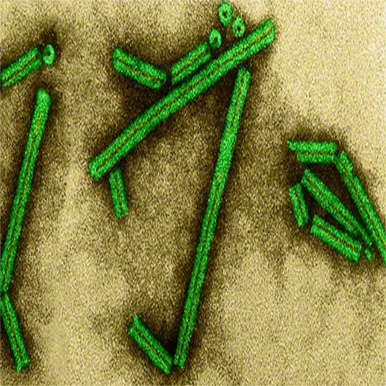
\includegraphics[height=2.25cm]{tobaccomosaicvirus} \\
				tobacco mosaic virus \\
				$L\sim \SI{300}{nm}$ \\
				\par
			}
		\end{column}
	

	\end{columns}

	\begin{itemize}
		\item The ability to measure particle shape is highly desirable for sensing applications
 		\item How can we extend RP sensing to measure length in addition to volume?
 	\end{itemize}
	

\end{frame}




%%%%%%%%%%%%%%%%%%%%%%%%%%%%%%%%%%%%%%%%%%%%%%%%%%%%%%%%%%%%%%%%%%%%%%%%%%%%%%%%%%%%%%%%%%%%%%%%%%%%%%%%%%%%%%%%%%%%%%%%%%%%
% Length convolution explanation
%%%%%%%%%%%%%%%%%%%%%%%%%%%%%%%%%%%%%%%%%%%%%%%%%%%%%%%%%%%%%%%%%%%%%%%%%%%%%%%%%%%%%%%%%%%%%%%%%%%%%%%%%%%%%%%%%%%%%%%%%%%%

\begin{frame}[c]{Resistive pulse in non-constant width pores}
	\begin{itemize}
		\item Consider the RP amplitude for translocation through non-uniform pores
	\end{itemize}
	$$ \Delta R\left(z'\right)=\frac{\rho}{\pi}\left[\int_{z=z'}^{z=z'+l_{p}}\left(\frac{1}{r_{P}^{2}\left(z\right)-s_{p}^{2}\left(z\right)}-\frac{1}{r_{P}\left(z\right)^{2}}\right)dz\right] $$
	\begin{itemize}
		\item RP amplitude is a function of the pore geometry \textbf{local to the particle's position}
		\item Particles map the interior of the pore during translocation with their RP signal!
	\end{itemize}
	
	{\centering
		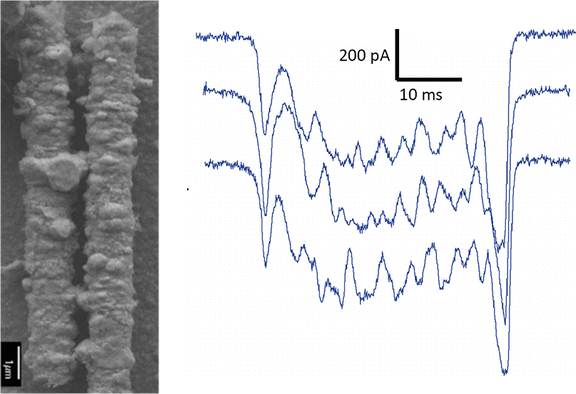
\includegraphics[width=2in]{particlesreveal.png} \\
		\par
	}

	
\end{frame}


%%%%%%%%%%%%%%%%%%%%%%%%%%%%%%%%%%%%%%%%%%%%%%%%%%%%%%%%%%%%%%%%%%%%%%%%%%%%%%%%%%%%%%%%%%%%%%%%%%%%%%%%%%%%%%%%%%%%%%%%%%%%
% Length convolution explanation
%%%%%%%%%%%%%%%%%%%%%%%%%%%%%%%%%%%%%%%%%%%%%%%%%%%%%%%%%%%%%%%%%%%%%%%%%%%%%%%%%%%%%%%%%%%%%%%%%%%%%%%%%%%%%%%%%%%%%%%%%%%%

\begin{frame}[c]{Resistive pulse in non-constant width pores}
	\begin{itemize}
		\item For particles with length shorter than characteristic length of changes in pore size, the interior is mapped with high resolution
		\item Long particles map pore interiors with low resolution because their lengths extend across multiple features
	\end{itemize}
	\vspace{.1in}
	$$ \Delta R\left(z'\right)=\frac{\rho}{\pi}\left[\int_{z=z'}^{z=z'+l_{p}}\left(\frac{1}{r_{P}^{2}\left(z\right)-s_{p}^{2}\left(z\right)}-\frac{1}{r_{P}\left(z\right)^{2}}\right)dz\right] $$
	\vspace{.1in}
	{\centering
		Simulated resistive pulses of short and long rods \\
		\vspace{.1in}
		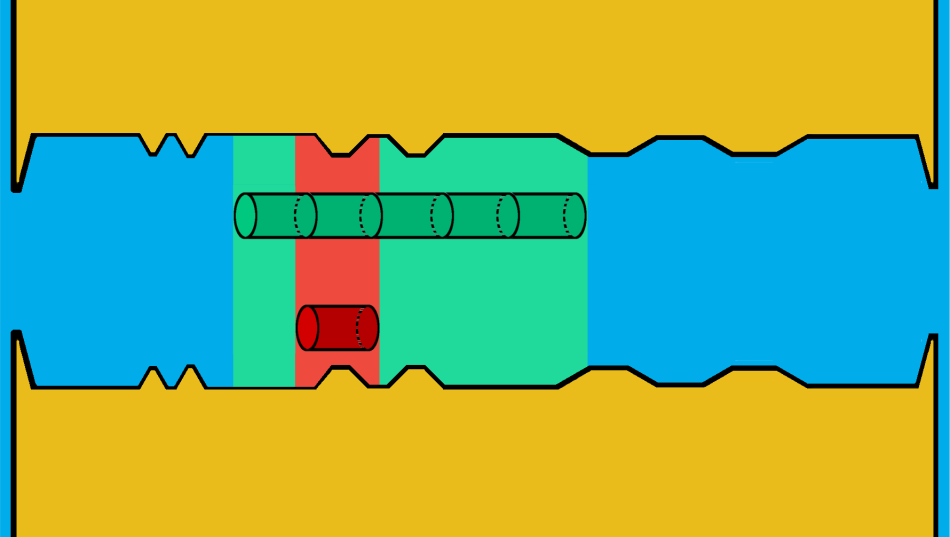
\includegraphics[height=1.05in]{rod_convolution.png}
		\hspace{.4in}
		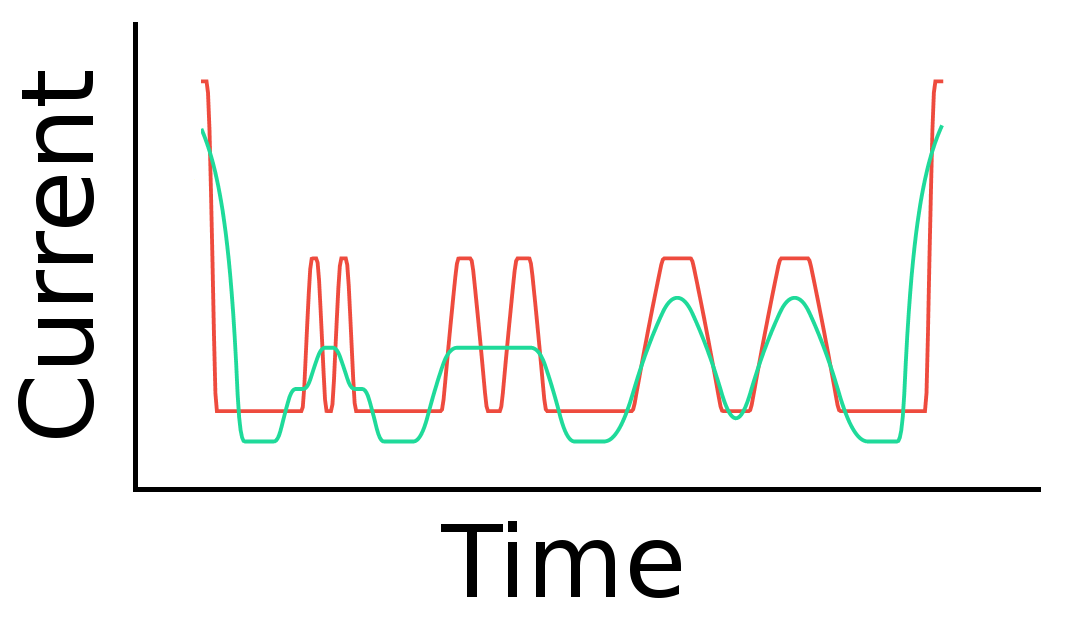
\includegraphics[height=1.05in]{rod_simulated_labeled.png}
		\par
	}
	
\end{frame}

%%%%%%%%%%%%%%%%%%%%%%%%%%%%%%%%%%%%%%%%%%%%%%%%%%%%%%%%%%%%%%%%%%%%%%%%%%%%%%%%%%%%%%%%%%%%%%%%%%%%%%%%%%%%%%%%%%%%%%%%%%%%
% Qualitative length measurement
%%%%%%%%%%%%%%%%%%%%%%%%%%%%%%%%%%%%%%%%%%%%%%%%%%%%%%%%%%%%%%%%%%%%%%%%%%%%%%%%%%%%%%%%%%%%%%%%%%%%%%%%%%%%%%%%%%%%%%%%%%%%

\begin{frame}[c]{Qualitative length measurement with resistive pulse}
	\begin{itemize}
		\item The 'resolution' of a resistive pulse signal provides a means of qualitatively determining particle length
		\item Short particles of known length can provide a high resolution mapping to compare with
		\item Qualitatively, the signals of longer particles should appear similar to the signals of shoter particles, but `smoothed out'
	
\end{frame}



%%%%%%%%%%%%%%%%%%%%%%%%%%%%%%%%%%%%%%%%%%%%%%%%%%%%%%%%%%%%%%%%%%%%%%%%%%%%%%%%%%%%%%%%%%%%%%%%%%%%%%%%%%%%%%%%%%%%%%%%%%%%
% Length measurement experimental platform
%%%%%%%%%%%%%%%%%%%%%%%%%%%%%%%%%%%%%%%%%%%%%%%%%%%%%%%%%%%%%%%%%%%%%%%%%%%%%%%%%%%%%%%%%%%%%%%%%%%%%%%%%%%%%%%%%%%%%%%%%%%%

\begin{frame}[c]{Length measurement experimental platform}
	\begin{itemize}
		\item Resistive pulses can be seen as a map of the pore interior for pores with non-constant radius
		\item In regions of low diameter, the pulse is deeper; in large diameter regions, the pulse is shallow
		\item Particles shorter than the length scale of diameter variation accurately map the pore interiors
		\item Particles longer than the length scale of diameter variation create RP signals that can be seen as a convolution of the pore's interior shape
	\end{itemize}
	
	\begin{equation}
		\begin{split}
			 \Delta R = R_{p}-R_{0} &= \rho\int_{z=0}^{z=l_{P}}\frac{dz}{A\left(z\right)}-\rho\int_{z=0}^{z=l_{P}}\frac{dz}{A'\left(z\right)} \\ 
			 &= \rho\int_{z=z'-l_{p}/2}^{z=z'+l_{p}/2}\frac{1}{\pi\left[r_{P}^{2}\left(z\right)-r_{p}^{2}\left(z\right)\right]}-\frac{1}{\pi r_{P}^{2}\left(z\right)}
		\end{split}
	\end{equation}

\end{frame}